%% ----------------------------------------------------------------
%% Thesis.tex
%% ---------------------------------------------------------------- 
\documentclass{ecsthesis}      % Use the Thesis Style
\graphicspath{{../Figures/}}   % Location of your graphics files
\usepackage{natbib}   
\usepackage{pdfpages}         % Use Natbib style for the refs.
\usepackage{enumitem} 
\usepackage{algpseudocode}
\newcommand{\params}[2]{$n_{\text{steps}}=#1,\ n_{\text{paths}}=#2$}
\usepackage[ruled,vlined]{algorithm2e}
\DontPrintSemicolon
\LinesNumberedHidden
\SetKwInOut{Input}{Input}
\SetKwInOut{Params}{Params}
\SetKwInOut{Output}{Output}

\hypersetup{colorlinks=false}   % Set to false for black/white printing
%% ----------------------------------------------------------------
%% Definitions.tex
%% ---------------------------------------------------------------- 
\newcommand{\BibTeX}{{\rm B\kern-.05em{\sc i\kern-.025em b}\kern-.08em T\kern-.1667em\lower.7ex\hbox{E}\kern-.125emX}}

%% People
\newcounter{address}
\setcounter{address}{1}
\renewcommand{\theaddress}{\textsuperscript{\fnsymbol{address}}}
\newcommand{\address}[1]{\refstepcounter{address}\theaddress#1\\}
\newcommand{\Name}[3]{\texorpdfstring{\href{mailto:#3}{#2}#1}{#2}\xspace}
\newcommand{\SteveRGunn}[1]{\Name{#1}{Steve R. Gunn}{S.R.Gunn@ecs.soton.ac.uk}}

%% Dingbats
\newcommand{\tick}{\ding{51}}
\newcommand{\cross}{\ding{55}}

%% Calculus
\newcommand{\pd}[2]{\ensuremath{\frac{\partial #1}{\partial #2}}\xspace}
\newcommand{\fd}[2]{\ensuremath{\frac{d #1}{d #2}}\xspace}
\newcommand{\dint}{\ensuremath{\int\!\!\!\int}\xspace}
\newcommand{\tint}{\ensuremath{\int\!\!\!\int\!\!\!\int}\xspace}

%% Math Sets
\newcommand{\Q}[1]{\ensuremath{\mathbb{#1}}\xspace}
\newcommand{\R}{\Q{R}}

%% Matrix, Vector
\newcommand{\V}[1]{\ensuremath{\boldsymbol{#1}}\xspace}
\newcommand{\M}[1]{\ensuremath{\boldsymbol{#1}}\xspace}
\newcommand{\0}{\V{0}}
\newcommand{\1}{\V{1}}
\newcommand{\I}{\M{I}}

%% Math Functions
\newcommand{\F}[1]{\ensuremath{\mathrm{#1}}\xspace}
\newcommand{\sgn}{\F{sgn}}
\newcommand{\tr}{\F{trace}}
\newcommand{\diag}{\F{diag}}

%% Math Names
\newcommand{\N}[1]{\ensuremath{\mathit{#1}}\xspace}

%% Data
\newcommand{\mc}[1]{\ensuremath{\mathcal{#1}}\xspace}
\newcommand{\Hyp}{\mc{H}}
\newcommand{\D}{\mc{D}}

%% Kernel
\newcommand{\K}{\M{K}}
\newcommand{\eins}{\texorpdfstring{\ensuremath{\epsilon}}{\textepsilon}-insensitive\xspace}
\newcommand{\e}{\ensuremath{\epsilon}\xspace}
\newcommand{\Bxi}{\ensuremath{\boldsymbol{\xi}}\xspace}
\newcommand{\Kanova}{\ensuremath{\mathit{K_{ANOVA}}}\xspace}
\newcommand{\Kspline}{\ensuremath{\mathit{K_{spline}}}\xspace}

%% Bayesian
\newcommand{\MP}{\ensuremath{\mathit{{\scriptscriptstyle \hspace{-1.5pt}M\hspace{-1.5pt}P}}}\xspace}
\newcommand{\ML}{\ensuremath{\mathit{{\scriptscriptstyle \hspace{-1.5pt}M\hspace{-1.5pt}L}}}\xspace}
\newcommand{\Qw}{\ensuremath{Q_{\w}(\w)}\xspace}
\newcommand{\Qa}{\ensuremath{Q_{\Ba}(\Ba)}\xspace}
\newcommand{\Qb}{\ensuremath{Q_{\beta}(\beta)}\xspace}
\newcommand{\wMPab}{\ensuremath{\w_{\MP|\bar {\Ba},\bar \beta}}\xspace}
\newcommand{\wMP}{\ensuremath{\w_{\MP}}\xspace}
\newcommand{\yMP}{\ensuremath{y_{\MP}}\xspace}
\newcommand{\BaMP}{\ensuremath{\Ba_{\hspace{1pt}\MP}}\xspace}
\newcommand{\aMP}{\ensuremath{\alpha_{\hspace{1pt}\MP}}\xspace}
\newcommand{\bMP}{\ensuremath{\beta_{\hspace{1pt}\MP}}\xspace}
\newcommand{\Sab}{\ensuremath{\M{\Sigma}_{\bar \Ba,\bar \beta}}\xspace}
\newcommand{\Ba}{\ensuremath{\boldsymbol{\alpha}}\xspace}
\newcommand{\Bb}{\ensuremath{\boldsymbol{\beta}}\xspace}
\newcommand{\Bm}{\ensuremath{\boldsymbol{\mu}}\xspace}
\newcommand{\BL}{\ensuremath{\boldsymbol{\Lambda}}\xspace}
\newcommand{\BPhi}{\ensuremath{\boldsymbol{\Phi}}\xspace}
\newcommand{\SMP}{\ensuremath{\M{\Sigma}_{\MP}}\xspace}

\newcommand{\Pa}{\ensuremath{P(\alpha|\mathcal{H})}\xspace}
\newcommand{\Pb}{\ensuremath{P(\beta|\mathcal{H})}\xspace}
\newcommand{\Pab}{\ensuremath{P(\alpha,\beta|\mathcal{H})}\xspace}
\newcommand{\Pw}{\ensuremath{P(\w|\mathcal{H})}\xspace}
\newcommand{\PD}{\ensuremath{P(\D|\mathcal{H})}\xspace}
\newcommand{\PwIa}{\ensuremath{P(\w|\alpha,\mathcal{H})}\xspace}
\newcommand{\PDIwb}{\ensuremath{P(\D|\w,\beta,\mathcal{H})}\xspace}
\newcommand{\PDwab}{\ensuremath{P(\D,\w,\alpha,\beta|\mathcal{H})}\xspace}
\newcommand{\PDIw}{\ensuremath{P(\D|\w,\mathcal{H})}\xspace}
\newcommand{\PwID}{\ensuremath{P(\w|\D,\mathcal{H})}\xspace}
\newcommand{\PwabID}{\ensuremath{P(\w,\alpha,\beta|\D,\mathcal{H})}\xspace}

\newcommand{\PanH}{\ensuremath{P(\alpha)}\xspace}
\newcommand{\PbnH}{\ensuremath{P(\beta)}\xspace}
\newcommand{\PabnH}{\ensuremath{P(\alpha,\beta)}\xspace}
\newcommand{\PwnH}{\ensuremath{P(\w)}\xspace}
\newcommand{\PDnH}{\ensuremath{P(\D)}\xspace}
\newcommand{\PwIanH}{\ensuremath{P(\w|\alpha)}\xspace}
\newcommand{\PDIwbnH}{\ensuremath{P(\D|\w,\beta)}\xspace}
\newcommand{\PDwabnH}{\ensuremath{P(\D,\w,\Ba,\beta)}\xspace}
\newcommand{\PDIwnH}{\ensuremath{P(\D|\w)}\xspace}
\newcommand{\PwIDnH}{\ensuremath{P(\w|\D)}\xspace}
\newcommand{\PwabIDnH}{\ensuremath{P(\w,\alpha,\beta|\D)}\xspace}

\newcommand{\PDwBab}{\ensuremath{P(\D,\w,\Ba,\beta|\mathcal{H})}\xspace}
\newcommand{\PwIBa}{\ensuremath{P(\w|\Ba,\mathcal{H})}\xspace}
\newcommand{\PBab}{\ensuremath{P(\Ba,\beta|\mathcal{H})}\xspace}
\newcommand{\PwBabID}{\ensuremath{P(\w,\Ba,\beta|\D,\mathcal{H})}\xspace}

\newcommand{\PBanH}{\ensuremath{P(\Ba)}\xspace}
\newcommand{\PwIBanH}{\ensuremath{P(\w|\Ba)}\xspace}

%% Snakes
\newcommand{\Esnake}{\ensuremath{\mathit{E_{snake}}}\xspace}
\newcommand{\Eimage}{\ensuremath{\mathit{E_{image}}}\xspace}
\newcommand{\Econt}{\ensuremath{\mathit{E_{cont}}}\xspace}
\newcommand{\Ecurv}{\ensuremath{\mathit{E_{curv}}}\xspace}
\newcommand{\Eint}{\ensuremath{\mathit{E_{int}}}\xspace}
\newcommand{\Eext}{\ensuremath{\mathit{E_{ext}}}\xspace}
\newcommand{\Eterm}{\ensuremath{\mathit{E_{term}}}\xspace}
\newcommand{\Eline}{\ensuremath{\mathit{E_{line}}}\xspace}
\newcommand{\Eedge}{\ensuremath{\mathit{E_{edge}}}\xspace}
\newcommand{\Econ}{\ensuremath{\mathit{E_{con}}}\xspace}
\newcommand{\Eangle}{\ensuremath{\mathit{E_{angle}}}\xspace}
\newcommand{\Elshape}{\ensuremath{\mathit{E_{lshape}}}\xspace}
\newcommand{\Eedgedir}{\ensuremath{\mathit{E_{edgedir}}}\xspace}
\newcommand{\Emodel}{\ensuremath{\mathit{E_{model}}}\xspace}
\newcommand{\wte}{\ensuremath{\mathit{w_{term}}}\xspace}
\newcommand{\wli}{\ensuremath{\mathit{w_{line}}}\xspace}
\newcommand{\wed}{\ensuremath{\mathit{w_{edge}}}\xspace}
\newcommand{\wco}{\ensuremath{\mathit{w_{con}}}\xspace}

%% Environments
\newcounter{alg}
\iffalse
\newenvironment{algorithm}[1]
{
    \stepcounter{alg}
    \begin{table}[htb]
    \centering
    \begin{tabular}[t]{ll}
    \hline&\\
    \multicolumn{2}{l}{\bf Algorithm \arabic{alg}: #1}\\&\\
} {
    &\\
    \hline
    \end{tabular}
    \end{table}
}
\fi            % Include your abbreviations

%% ----------------------------------------------------------------
\begin{document}
\frontmatter
\title      {Signature-Kernel Regime Detection and a Regime-Aware Lead–Lag Overlay}
\addresses  {\groupname {Faculty of Social Sciences}\\
	         \deptname {Mathematics School}\\ 
	         \univname {University of Southampton}}

\authors    {\texorpdfstring
{\href{}{Zhe GUAN}}
{3-36516473}
}
\date       {\today}
\supervisor {Sasan Barak}
\examiner {}

\subject    {Mathemetics}
\keywords   {}
\maketitle
\begin{abstract}

This dissertation studies lead--lag structure in the cryptocurrency market and its use for return prediction and portfolio construction. Rolling directed lead--lag matrices are built with a signature (sequence–kernel) estimator on 30 business–day windows (update every day, maximum lag 7) after winsorizing daily returns at the 2.5/97.5\% tails. A baseline long–short hedge goes long “followers” and short “leaders” identified by row–mean scores. A strict walk–forward regime detector is then introduced: Bitcoin path groups are compared using a signature–kernel MMD distance, clustered on historical data under a visibility constraint, mapped to bear/neutral/bull, and compressed to a daily regime by a rolling vote. The trading overlay conditions the baseline by the sign of each asset’s relation to the anchor and applies a fixed neutral scaling ($\alpha=0.5$) while preserving the baseline hedge.

The dataset contains daily closes for 72 Binance–listed assets from 2021-01 to 2024-06. At the same time–in–market (43\%), the regime overlay improves headline performance relative to the baseline: cumulative return 132.8\% vs.\ 59.5\%, CAGR 31.4\% vs.\ 16.3\%, Sharpe 1.46 vs.\ 0.58, annualized volatility 20.1\% vs.\ 38.1\%, and maximum drawdown $-14.2\%$ vs.\ $-35.3\%$ (pre–costs). It outperforms in three of four calendar years and turns a negative 2023 baseline (-5.42\%) into a positive outcome (+7.79\%). Robustness checks across estimator variants and parameter settings indicate stable signals; performance declines when detection and rebalancing are less frequent, consistent with slow information diffusion. Data–driven leaders and followers show limited overlap with size/volume rankings, suggesting the structure is not a capitalization effect.

\textbf{Keywords:} lead--lag, return prediction, portfolio construction, regime detection, signature kernel, MMD, cryptocurrencies.

\iffalse
 This project builds and tests a market-neutral trading strategy that uses lead–lag relationships between cryptocurrencies.

 We generate rolling lead–lag matrices with different methods — Pearson correlation, distance correlation, and path signature — to see how well each one picks up directional influence between assets.
Among these, the signature-based method stands out for being more responsive to changing relationships, especially in volatile markets.

To make the strategy adapt to market conditions, we add a regime detection step that clusters sliding price segments into bull, bear, or neutral regimes, without using any future data.
This regime signal is then used to change how the strategy goes long and short depending on the market state.

Backtests on a basket of popular cryptocurrencies from January 2021 to June 2024 show that adding the regime signal improves results for all the lead–lag methods, with a clear boost in risk-adjusted returns when BTC is included.

We also run sensitivity checks, add a basic benchmark strategy for comparison, and keep the code modular for easy reuse.
\fi

\end{abstract}
\acknowledgements{Completing this master’s dissertation has been both an academic challenge and a personal milestone. Coming from a physics background, taking a first step into data–driven finance has felt like a small but meaningful achievement. I am grateful to everyone who helped make that transition possible.

I would like to express my sincere thanks to my supervisor, \textbf{Dr.\ Sasan Barak}, for clear guidance, steady support, and timely, constructive feedback at every stage. His encouragement to test ideas rigorously and try new methods helped me navigate the technical parts of this project and sharpen my analytical thinking.

I am deeply thankful to my parents for giving me the opportunity to study in the UK and for their constant support, both practical and emotional. 

Finally, thank you to my friends in Southampton for the long study sessions, dissertation discussions, and all the small moments that made this year memorable. Any remaining errors are my own.}

\includepdf[offset=25mm -30mm]{soo.pdf}
\tableofcontents
\listoffigures
\listoftables
\lstlistoflistings
%\listofsymbols{|l|l|}{
%BTC & Bitcoin \\
%S\&P &Standard \& Poor’s 500 Index
%\\$w$ & The weight vector}
\listofsymbols{|l|l|}{
AMH & Adaptive Markets Hypothesis \\
EMH & Efficient Market Hypothesis \\
TSMOM & Time-Series Momentum \\
FX & Foreign Exchange \\
RCM & Regime Classification Measure \\
DGP & Data-Generating Process \\
ARCH & Autoregressive Conditional Heteroskedasticity \\
GARCH & Generalized ARCH \\
SWARCH & Markov-Switching ARCH \\
NYSE & New York Stock Exchange \\
S\&P 500 & Standard \& Poor’s 500 Index \\
S\&P Composite & Standard \& Poor’s Composite Index \\
FTSE 100 & Financial Times Stock Exchange 100 Index \\
CAC 40 & Cotation Assistée en Continu 40 (French equity index) \\
ECM & Error-Correction Model \\
COC & Cost of Carry \\
ECM-COC & Error-Correction Model with Cost of Carry \\
ARMA & Autoregressive Moving-Average \\
VAR & Vector Autoregression \\
RMSE & Root Mean Squared Error \\
MAE & Mean Absolute Error \\
LLR & Lead–Lag Ratio \\
HY & Hayashi–Yoshida (estimator / cross-correlation) \\
CET & Central European Time \\
CAPM & Capital Asset Pricing Model \\
FF3 & Fama–French Three-Factor Model \\
FF5 & Fama–French Five-Factor Model \\
SBM & Stochastic Block Model \\
DI\text{-}SIM & Directed Spectral Clustering method (DI-SIM) \\
CCF & Cross-Correlation Function \\
AUC & Area Under the Curve \\
ARI & Adjusted Rand Index \\
MI & Mutual Information
BTC & Bitcoin (anchor asset)\\
WF & Walk–forward (rolling forward)\\
MMD & Maximum Mean Discrepancy\\
RBF & Radial Basis Function\\
NaN & Not a Number (missing value)\\
Inf & Infinity\\
bdays & Business days\\
$z_t$ & Daily market regime label (0=bear, 1=neutral, 2=bull)\\
$p_\tau$ & BTC close price at time $\tau$\\
$\gamma$ & Path embedding $\{(\tau,p_\tau)\}$\\
$\widehat\gamma$ & Transformed path $T(\gamma)$\\
$T$ & Path transformer (level standardization, time normalization)\\
$n_{\text{steps}}$ & Subpath length (number of steps)\\
$n_{\text{paths}}$ & Number of subpaths per group\\
$o$ & Overlap offset in subpath stride\\
$G_g$ & The $g$-th path group\\
$[s_g,e_g]$ & Calendar span covered by group $G_g$\\
$K_\Sigma$ & Signature kernel\\
$\Phi(\cdot)$ & Feature map induced by $K_\Sigma$\\
$\sigma$ & RBF bandwidth\\
$d$ & Dyadic order\\
$\lambda$ & Regularization parameter\\
$D_{g,h}$ & Group distance $\mathrm{MMD}(G_g,G_h)$\\
$D$ & Precomputed distance matrix $\in\mathbb{R}^{G\times G}$\\
$w$ & WF history window length (in groups)\\
$H$ & Forward horizon (days)\\
$n_c$ & Number of clusters\\
$\tau_{+},\tau_{-}$ & Thresholds for semantic mapping (bull/bear)\\
$E_g$ & Eligible history set at decision $g$\\
$m_c$ & Medoid of cluster $c$\\
$\mu_c$ & Mean $H$-day forward return of cluster $c$\\
$\psi(\cdot)$ & Mapping from cluster to \{bear, neutral, bull\}\\
$\mathrm{dir\_label}_g$ & Directional label of group $G_g$ ($\in\{0,1,2\}$)\\
$k$ & Count parameter: daily voting window size / minimum names (context-dependent)\\
$L$ & Rolling window length (bdays)\\
$f$ & Update/rebalance spacing (bdays)\\
$\ell_{\max}$ & Maximum forward lag\\
$m$ & Signature truncation order\\
$\mathcal{T}$ & Set of update dates\\
$N$ & Number of assets\\
$P_{i,t}$ & Close price of asset $i$ on day $t$\\
$r_{i,t}$ & Log return of asset $i$ on day $t$\\
$M_t$ & Signature-based lead–lag directed matrix at date $t$\\
$x^{(t,\ell)}_{i}$ & Past sequence of $i$ on $W_t$ (aligned to $j$’s future)\\
$y^{(t,\ell)}_{j}$ & Future sequence of $j$ on $W_t$ (shifted by $\ell$)\\
$\Phi_m(\cdot)$ & Signature feature vector up to order $m$\\
$\widehat\Phi_m(\cdot)$ & Normalized signature features\\
$s^{(\ell)}_{ij}(t)$ & Directional similarity score (“$i$ then $j$” minus “$j$ then $i$”)\\
$\ell^\star_{ij}(t)$ & Lag maximizing $|s^{(\ell)}_{ij}(t)|$\\
$s_t(i)$ & Row-mean leadership score of asset $i$\\
$\mathcal{L}_t,\ \mathcal{F}_t$ & Leaders / followers sets (by quantiles)\\
$Q_q(\cdot)$ & Quantile operator (the $q$-quantile)\\
$w_{t^+}(i)$ & Portfolio weight of asset $i$ executed on $t^+$\\
$R_{t^+}$ & Baseline strategy daily return realized on $t^+$\\
$a$ & Anchor asset (here $a=\mathrm{BTC}$)\\
$\mathrm{rel}_t(i)$ & Signed anchor relation for asset $i$ (from $M_t$)\\
$\mathcal{B}^{\mathrm{long}},\ \mathcal{B}^{\mathrm{short}}$ & Long / short baskets\\
$\mathcal{F}_t^{+},\ \mathcal{F}_t^{-}$ & Followers with $\mathrm{rel}_t(i)>0$ / $<0$\\
$\mathcal{L}_t^{+},\ \mathcal{L}_t^{-}$ & Leaders with $\mathrm{rel}_t(i)>0$ / $<0$\\
$R^{\mathrm{overlay}}_{t^+}$ & Regime-aware overlay daily return\\
$\alpha$ & Neutral-period scaling coefficient (set to $0.5$)\\
$\overline{r}_{\mathcal{B},\,t^+}$ & Average return of basket $\mathcal{B}$ on $t^+$\\
$t^+$ & Next trading day (relative to update date $t$)\\
$\mathcal{U}$ & Investable universe / tradable asset set
}

\mainmatter
%% ----------------------------------------------------------------
%% ----------------------------------------------------------------
%% Introduction.tex
%% ---------------------------------------------------------------- 
\chapter{Introduction} \label{Chapter:Introduction}

This dissertation was a part of my master’s project at the Univerisity of Southampton, under the guidance of Dr. Sasan Barak. The project focuses on financial data science within cryptocurrency markets. 

Financial markets, like cryptocurrencies, are widely considered to be non-stationary~\cite{Schmitt_2013,Lo} as their statistical properties—including volatility, correlations, and return distributions change frequently over time.
The non-stationarity brings a major challenge for trading and risk management, as optimised strategies under one regime often fail when market condition changes~\cite{10.1093/rfs/15.4.1137}. 

Traditional trading strategies generally assume a stable market environment, therefore the strategy performance probably varies across different market states. For example, a momentum-based method may perform well in a trending market but much worse in volatile periods~\cite{MOSKOWITZ2012228}; Similarly, risk measures calculated under a volatility regime may underestimate the risk during a crisis regime~\cite{HAMILTON1994307}.

To address the challenges from market non-stationarity, a range of methods are developed, such as Markov switching models~\cite{hamilton1989new}, and clustering approaches~\cite{10.1093/rfs/15.4.1137}. More recently, mathematical tools from rough path theory have given rise to signature methods~\cite{ chevyrev2025primersignaturemethodmachine,issa2023nonparametriconlinemarketregime}, which are capable of extracting rich path-wise features from time series data. Combined with clustering, these features can be used to identify distinct market regimes, such as bull, bear, and neutral phases.

In this study, we applied signature methods~\cite{Lyons1998, chevyrev2025primersignaturemethodmachine,issa2023nonparametriconlinemarketregime} to extract path-wise features from BTC prices and perform walk-forward clustering to obtain bull/neutral/bear regimes. We then applied a cross-sectional lead–lag hedge~\cite{lyons2002system, gatheral2018volatility} as the baseline and overlay the regime signal to adjust position signs and exposure.


The main contributions of this dissertation can be summarised in three parts. First, it shows how signature methods can be used for regime detection in cryptocurrency markets, which is still a relatively new application. Second, it develops a framework that combines regime signals with trading strategies, taking the lead–lag strategy as the baseline. Third, it provides a comparative evaluation between the baseline strategy and its regime-aware extension, showing the benefits in risk–return trade-offs as well as the limits of the application.

The dissertation is organised as follows. Chapter 2 reviews the relevant literature on financial market non-stationarity, regime detection methods, and cryptocurrency trading strategies. Chapter 3 introduces the methodology, including signature methods, clustering techniques, and the construction of baseline and regime-aware strategies. Chapter 4 presents the empirical results and performance evaluation. Chapter 5 discusses the limitations and potential extensions, including multi-asset regimes and transaction cost considerations. Finally, Chapter 6 concludes with a summary of contributions and directions for future research.

%The lead–lag effect \cite{Podobnik_2010} is about timing — when changes in one time series tend to show up before similar changes in another. An illustration of this in financial markets is that some assets shows predictable movements because their price changes tend to follow those of other assets after a certain time lag \cite{huth2012highfrequencyleadlagrelationships,repec:taf:quantf:v:18:y:2018:i:5:p:725-735}. The study of lead-lag relationships between asset returns can help active investors build trading algorithms that exploit the time lag in the movement of one asset relative to another and generate strong returns \cite{Li2022}.

\iffalse
Many methods are developed to detect the lead-lag relationship

You probably found all the files from \cite{Gunn:2001:pdflatex}.
\tref{Table:tabex} illustrates the results of my work.
\begin{table}[!htb]
  \centering
  \begin{tabular}{cc}
  \toprule
  \textbf{Training Error} & \textbf{Testing Error}\\
  \midrule
  0 & $\infty$\\
  \bottomrule
  \end{tabular}
  \caption{The Results}
  \label{Table:tabex}
\end{table}

\fref{Figure:figex} shows why this is the case.
\begin{figure}[!htb]
  \centering
  
\includegraphics[width=8cm]{figure}
  \caption{A colourful picture.}
  \label{Figure:figex}
\end{figure}

This page shows you a subfigure example in \fref{Figure:figsubex}.
\begin{figure}[!htb]
  \centering
  \subfigure[The left caption]{
    
\includegraphics[width=4.2cm]{figure}
    \label{Figure:figsubex:left}
  }
  \subfigure[The right caption]{
    
\includegraphics[width=4.2cm]{figure}
    \label{Figure:figsubex:right}
  }
  \caption{A doubly colourful picture.}
  \label{Figure:figsubex}
\end{figure}
\fi
%% ----------------------------------------------------------------
%% Conclusions.tex
%% ---------------------------------------------------------------- 

\chapter{Literature Review} \label{Chapter: Conclusions}

\section{Non-stationarity in Financial Markets}

Non-stationarity is a defining feature of financial returns. In practice, the conditional mean, the variance, the higher moments, and the cross-sectional dependence structure evolve over time as market composition, policy, and technology change. Accordingly, this subsection organises the literature into four strands that motivate our empirical design. First, time-varying covariances can generate heavy tails. Second, adaptive market dynamics imply state- and time-dependent predictability. Third, cross-asset time-series momentum provides evidence of time-varying serial dependence. Fourth, volatility often switches across regimes. Consistent with these strands, we emphasise approaches that model non-stationarity explicitly, such as Markov switching and time-varying volatility. We also emphasise approaches that infer non-stationarity non-parametrically via rolling windows and clustering. Finally, we relate these ideas to our later use of \emph{path-wise} signature features and strict walk-forward clustering for regime identification.


\cite{Schmitt_2013} place non-stationarity at the center of their analysis. The authors study 306 continuously traded S\&P 500 stocks from 1992--2012. In rolling windows, they show that volatilities and correlations vary strongly over time. When the covariance matrix is held fixed over short windows, multivariate returns appear approximately Gaussian. To capture the fact that covariances fluctuate, the authors replace the fixed covariance with a Wishart random matrix. This substitution yields an ensemble-averaged return distribution governed by a single parameter $N$, which measures the strength of correlation and covariance fluctuations. A smaller $N$ indicates stronger non-stationarity and heavier tails. As $N \rightarrow \infty$, the model approaches Gaussian behaviour. Empirically, the model fits the market-wide return distribution well and attributes heavy tails to time-varying covariances. The estimated $N$ rises with the return horizon. The estimate is about $N \approx 5$ for daily returns and about $N \approx 14$ for 20-day returns. This pattern implies that non-stationarity is stronger at short horizons. However, some deviations remain in the extreme tails. The study does not address the underlying economic mechanisms. Even so, the framework provides a consistent way to capture heavy tails through covariance non-stationarity.


\cite{Lo} places non-stationarity at the core of the Adaptive Markets Hypothesis (AMH). In this view, market efficiency changes over time as the market ecology evolves. Moreover, the risk-return relation changes as conditions shift. Likewise, the equity risk premium and strategy profitability change with the environment. Specifically, the ecology includes participants, institutions, and regulation, which shift continually. Consequently, empirical relationships are time-varying and path-dependent rather than fixed. Within this framework, arbitrage opportunities emerge and disappear. Strategies wax and wane as conditions change. Thus, the AMH replaces the EMH's stationary convergence with cycles, trends, and episodes of panic and recovery. For evidence, a rolling five-year first-order autocorrelation for the S\&P Composite (1871-2003) shows cyclical efficiency. The pattern does not march monotonically toward zero autocorrelation. Hence, the result challenges stationary-equilibrium implementations of the EMH. Practically, the model implies that adaptation and innovation are necessary responses to a changing environment. Accordingly, survival rather than static optimality becomes the organising objective. Finally, the AMH interprets behavioural regularities as evolutionary heuristics whose market impact varies with population composition. Moreover, emotion and selection shape which agents remain active. Taken together, these features provide additional evidence that the data-generating process is non-stationary.


Similarly, \cite{MOSKOWITZ2012228} study 58 liquid futures and forwards across equities, FX, commodities, and government bonds. The sample covers mainly 1985–2009. For comparability, the authors scale positions by ex-ante volatility. Consequently, the authors document strong 1-12-month continuation followed by partial multi-year reversal. Moreover, a diversified TSMOM factor delivers large alphas relative to standard equity factors and ``everywhere'' factors. The factor performs best in extreme markets. Hence, the payoffs appear state-dependent. In a formal decomposition, the authors attribute profits mainly to positive auto-covariance, which reflects time-series dependence. By contrast, the cross-asset lead-lag and mean-return components are small or even negative. In addition, position data show that speculators ride trends, whereas hedgers take the other side. Finally, these patterns support a non-stationary, state-dependent return-generating process rather than one with constant parameters.


In line with the above evidence on non-stationarity, \cite{HAMILTON1994307} replace a stationary GARCH view with a Markov-switching ARCH (SWARCH) specification. The specification lets volatility parameters jump across latent regimes. The authors estimate the model on weekly NYSE value-weighted returns from 1962 to 1987. The model allows 2-4 regimes and student's $t$ innovations with a leverage term. The results show that standard GARCH overstates persistence and forecasts poorly. By contrast, SWARCH captures discrete regime shifts. The shifts include quiet, moderate, high, and an extreme state that isolates the October 1987 crash. The model improves short- and multi-week variance forecasts, especially for the four-state case. The paper also reframes persistence. The authors interpret persistence as state persistence, meaning long-lived regimes, rather than the slow decay of shocks. Once regime changes are modelled, the ARCH component becomes much less persistent. High-volatility states line up with business recessions. Negative returns raise volatility more than equal-size positive returns, which confirms leverage. These patterns further underscore time variation in the data-generating process. Overall, the paper treats equity volatility as a regime-switching, non-stationary phenomenon. Consequently, the framework yields cleaner inference and better forecasts than stationary ARCH/GARCH benchmarks.

Taken together, these strands support an empirical design. The design treats regimes as evolving objects and detects regimes from data rather than imposing them \emph{ex ante}. Accordingly, our approach uses signature-based path features. Our approach also applies strict walk-forward clustering. Together, these tools yield daily bull, neutral, and bear states. We then condition a cross-sectional lead-lag hedge on those states.

\section{Path Signatures for Sequential Data}

A \emph{path signature} is an infinite, ordered list of iterated integrals\cite{issa2023nonparametriconlinemarketregime}. The signature captures both the shape and the time ordering of a multivariate path. The concept comes from rough path theory. \cite{Lyons1998} formalise the signature as a unique encoding up to time reparameterisation. The representation is non-parametric and coordinate-free.
For a path $X:[0,T]\to\mathbb{R}^d$, the $k$-th level is
\[
S^{(k)}(X)
=\int_{0<t_1<\cdots<t_k<T} dX_{t_1}\otimes\cdots\otimes dX_{t_k}.
\]
This term is a tensor in $(\mathbb{R}^d)^{\otimes k}$. The level collects all $k$-fold, time-ordered integrals. These levels encode increments, signed areas, and higher-order interactions. Consequently, the signature summarises how the path evolves through time, not only where it ends. The signature is invariant to the speed of traversal, and also obeys key algebraic laws. The \emph{shuffle product} and \emph{Chen's identity} link products and concatenations of paths \cite{https://doi.org/10.1112/plms/s3-4.1.502}. These laws give the object a rich and tractable structure. A truncation at order $m$ yields a finite feature vector. The vector summarises the path up to order-$m$ effects. Thus, the signature provides practical features with clear theoretical meaning.

Over the past decade, path signatures have moved to the forefront of machine learning for sequential data. Lyons and collaborators have led this shift. A growing body of work shows that signature features are powerful inputs for time-series classification and prediction. For example, \cite{chevyrev2025primersignaturemethodmachine} provides a concise primer. The authors highlight reparameterisation invariance, the existence of a log-signature in a free Lie algebra, and a universal approximation view. Consequently, the properties justify using signatures as a basis for feature learning. In practice, standard pipelines follow three steps. One first embeds raw discrete observations into a continuous path, for example via piecewise-linear interpolation. One then computes a truncated signature. The approximation result provides the key rationale. Polynomial functionals of a path reduce to linear functionals of signature terms. Therefore, a linear model on sufficiently high-order signature features can approximate any continuous functional on a suitable path space. This universality allows complex path dependence without manual feature engineering. Instead, the model learns weights on signature terms.


For financial applications, the second-order signature terms represent \emph{areas} spanned by pairs of variables over time. These signed areas encode temporal ordering information. Consequently, researchers use these areas as measures of lead-lag or causal asymmetry between time series. For instance, if an asset $A$ consistently loops ahead of another asset $B$ in price-path space, the signed area becomes large. This pattern implies that $A$ tends to lead $B$. Moreover, \cite{bennett2022leadlag} include a rough-path signature \emph{area} term in their lead--lag correlation measures. Likewise, \cite{repec:taf:quantf:v:17:y:2017:i:6:p:959-977} proposes a hypothesis test for lag/lead relations based on the statistical significance of the signed area between two time series. Taken together, these applications show that path signatures detect subtle time-directed dependencies. Standard correlation or cross-covariance methods often miss such effects.


Another advantage is that signatures combine naturally with kernel methods. In particular, the \emph{signature kernel} defines an inner product between signature feature maps. The kernel enables efficient comparison of paths in a high-dimensional feature space. The approach avoids explicit truncation of the signature. Building on this idea, \cite{issa2023nonparametriconlinemarketregime} develop an online two-sample test for regime shifts. The test uses signature features as the basis for a maximum mean discrepancy (MMD) statistic. Consequently, the method can flag, and flag quickly, when the distribution of recent market data departs from that of the past. More broadly, signature features capture fine-grained sequential structure and coarse aggregate effects. Therefore, the approach suits non-stationary financial problems.Accordingly, the remainder of this thesis will use path signature features via the signature kernel. We will embed asset price trajectories into a feature space. We will identify regimes and measure lead--lag effects in that space. Finally, we will remain agnostic about specific functional forms of dependence while exploiting the properties above.


\section{Approaches to Regime Detection}

Regime detection methods broadly fall into two families. \emph{Parametric} models posit a finite set of latent states with state-dependent moments and Markovian transitions. As a result, these models yield smoothed or filtered state probabilities and transition matrices that aid forecasting. By contrast, \emph{non-parametric} approaches infer state changes directly from the data's geometry. These approaches typically use rolling windows, distances or kernels, and clustering. Therefore, non-parametric methods relax distributional and Markov assumptions and also facilitate online updates. In our review, we compare methods along five dimensions. We consider modelling assumptions, estimation mode (batch vs.\ online and leakage control), output type (hard labels vs.\ probabilities), scalability to multivariate paths, and interpretability for portfolio use.

\cite{10.1093/rfs/15.4.1137} specify regimes as latent states of a multivariate normal DGP with state-dependent means, volatilities, and correlations. The authors infer regimes and transition probabilities via the Hamilton/Gray filter. The authors summarise classification quality with the Regime Classification Measure (RCM). The model recovers economically interpretable states; for example, the model finds a persistent high-volatility, high-correlation bear state and a lower-risk normal state. The model also reproduces downturn exceedance correlations where Gaussian and asymmetric GARCH fail. Key strengths include probabilistic outputs, expected durations, and tractable forecasts. However, key trade-offs include reliance on parametric structure, often with constant transition probabilities, and misspecification risk when the true dynamics deviate from a finite-state Markov chain.

\cite{issa2023nonparametriconlinemarketregime} develop an online regime detector on \emph{path space} using a two-sample MMD with rough-path signatures as features. The method uses the \emph{signature kernel} to compare paths. The pipeline ingests small streaming batches for fast reactivity. The pipeline scales to multidimensional series and handles non-Markovian, path-dependent structure. A rank-2 variant incorporates filtration (conditional) information. A kernel-trick implementation avoids explicit signature truncation. The same machinery also supports clustering and outlier detection. The demonstrations cover synthetic data and real markets, including equity baskets and crypto. The main appeal is minimal modelling assumptions and online operation. The main cost is that outputs are often hard labels or distance-based scores without an explicit transition model.

\cite{chevyrev2025primersignaturemethodmachine} provide a concise primer on path signatures. The authors describe signatures as an infinite sequence of iterated integrals that compactly capture time ordering. Core properties include time-reparametrisation invariance, the shuffle product, Chen's identities, time reversal, and the log-signature. These properties justify signatures as non-parametric feature maps for sequential data. A practical pipeline follows a simple flow: data $\rightarrow$ path $\rightarrow$ signature $\rightarrow$ features $\rightarrow$ learning. In many cases, second-order (area-type) terms improve class separability and extend naturally to multivariate time series. Linear functionals of signature terms approximate continuous functionals on compact path sets. Hence, signature features provide a principled basis for often linear models.

Guided by the above evidence, we adopt a non-parametric and \emph{strictly walk-forward} design. Our procedure embeds BTC paths via the signature kernel. Our rolling group distances then feed a clustering step on \emph{eligible history} only. Our mapping step assigns clusters to bull, neutral, or bear using forward $H$-day effects. Our voting step converts hard labels into a daily series via a $k$-vote. Compared with Markov-switching models, our design avoids parametric transition assumptions and emphasises leakage control. Compared with generic online detectors, our design targets portfolio use by tying cluster semantics to forward returns and by conditioning a cross-sectional lead--lag hedge on the detected state.


\section{Clustering-Based Regime Identification}

Beyond model-based switching frameworks, researchers identify market regimes with \emph{unsupervised clustering} of historical data. These approaches partition time periods into groups with internally similar characteristics. The characteristics often include return distributions and volatility levels. These methods do not require an explicit likelihood or a Markov structure. The main advantage is that clustering makes minimal assumptions about dynamics. As a result, clustering can detect novel or irregular regimes. The main challenge is that clustering typically produces hard classifications with no inherent temporal continuity. Unless researchers add an exogenous transition process, the labels do not evolve smoothly. Nevertheless, prior studies show that clustering can uncover economically meaningful states in financial markets.

One influential example is the Wasserstein $k$-means algorithm proposed by \cite{Horvath_2021, Horvath2024JCF}. This method treats each time window as a distribution. This method then clusters windows using the $p$-Wasserstein distance between empirical return distributions. This design contrasts with classical $k$-means, which clusters raw returns by Euclidean distance. Because the method considers the full distributional shape, the method is robust to heavy tails and skewness. The authors show that Wasserstein $k$-means can detect distinct market phases in an unsupervised fashion. The authors also show that the method significantly outperforms classical $k$-means and other baselines in separating regimes. The resulting clusters correspond to intuitive states, such as low-volatility and high-volatility regimes. Importantly, the method achieves this separation without a parametric state model. Follow-up work validates the method by computing maximum mean discrepancy scores between clusters. These studies confirm that the distributional differences are statistically significant. In both simulations and real financial time series, the Wasserstein clustering distinguishes regime segments reliably. In addition, the method adapts more flexibly than models that assume Gaussian returns or fixed transition probabilities.

Clustering methods can also incorporate cross-sectional information. \cite{10.1007/978-3-031-12426-6_1} argue that many regime detectors cannot identify new regimes on the fly or ignore relationships across assets. The authors propose a dynamic clustering model that jointly learns regime assignments for multiple time series while allowing time-varying transition probabilities. The idea is to group time periods by common cross-asset behaviour rather than by univariate patterns. This design yields cross-sectional regimes that improve multi-asset return forecasts. In this framework, regimes emerge as clusters of high-dimensional observations across assets. A flexible transition mechanism then captures how these clusters evolve. This line of work underscores the breadth of clustering approaches. The spectrum runs from simple rolling-window similarity checks to sophisticated high-dimensional models. The shared goal is to let the data speak for itself about regime structure.

Another related strand is non-parametric change-point detection. Researchers can view this strand as clustering with implicit two-segment clusters, namely pre-break and post-break. \cite{Matteson2014} develop an e-divisive means algorithm to detect multiple change points in multivariate series without parametric distributional assumptions. The method identifies points where the distribution shifts and thereby segments the series into distinct regimes. These techniques complement clustering. Whereas clustering often groups windows that need not be contiguous in time, change-point methods explicitly seek contiguous regime segments. Practitioners can also combine the two ideas by first detecting candidate breakpoints and then clustering segments.

Clustering-based methods typically output hard labels rather than smoothed probabilities. This property yields clear ex-post identification of regimes. However, this property also requires care in online or trading contexts to avoid lookahead bias. Many studies perform clustering on an entire historical sample or use rolling re-training that inadvertently uses future information. For practical trading signals, a strict walk-forward implementation is necessary. Such an implementation must use only information that is available at the decision time. Our design follows this principle by using an expanding window for clustering. Our design does not re-label past data when new data arrives. Our design defines regimes via forward-looking returns on a training set and then applies those definitions prospectively.

Clustering methods generally do not attach economic semantics to regimes by default. Users usually attach semantics by examining cluster characteristics, such as high volatility or large drawdowns, and then assigning names. Our approach bridges this gap by mapping clusters to bull, neutral, or bear labels based on forward $H$-day return outcomes in a training period. This mapping injects an economic interpretation directly into the clustering output. Thus, our approach forms a hybrid. The hybrid combines unsupervised identification of patterns with a supervised labeling step based on subsequent performance. This blend, together with strict walk-forward operation, aims to harness the adaptability of clustering while making the results usable in a live strategy.

\section{Lead--Lag Signals and Regime-Driven Overlay Trading Strategies}

Lead--lag captures a \emph{directed, time-shifted} dependence between assets. Specifically, the empirical evidence comes from two main strands. The first strand covers high-frequency studies that document futures-led price discovery and microstructure asymmetries. The second strand examines daily, multi-lag dependence that researchers organise as directed networks and convert into predictive signals. A recurring constraint in this literature is the role of \emph{trading frictions and execution latency}. These frictions determine whether statistical leadership translates into net returns. Accordingly, we summarise representative studies and we connect them to our regime-driven overlay design.

\cite{BROOKS200131} study FTSE~100 futures and cash with 10-minute data from 1996--1997. The authors first establish cointegration via Engle--Granger. The authors then estimate an error-correction model (ECM) and a cost-of-carry variant (ECM--COC) against ARMA and VAR benchmarks. Lagged futures returns significantly forecast spot returns. The carry-adjusted cointegration term is also significant. In a May 1997 hold-out, ECM--COC delivers the best out-of-sample accuracy with 68.75\% correct direction and the lowest RMSE and MAE. However, realistic round-trip costs (spot $\approx 1.70\%$, futures $\approx 0.116\%$) and a 10-minute execution delay remove the edge. Therefore, the key takeaway is clear. \emph{Futures lead price discovery, but frictions and latency can exhaust exploitable profits}.

\cite{huth2012leadlag} analyse CAC40 stocks and index futures with tick-by-tick data from March to May 2010. The authors use the \emph{Hayashi--Yoshida} correlation and an asymmetric lead--lag ratio (LLR). The simulations show that previous-tick estimators spuriously assign leadership to more active assets. The Hayashi--Yoshida estimator mitigates this bias. The empirical results show that futures lead constituents at sub-second lags with strong asymmetry (future/stock LLR $\approx 2$). The stock--stock links are weaker with peak lags near one second. The leadership aligns with liquidity through shorter intertrade durations, narrower spreads, lower midquote volatility, and higher turnover. The leadership also strengthens around macro releases and the U.S.\ open. A simple predictor that uses only the leader’s past yields about 60\% accuracy for the lagger’s next midquote change. Nevertheless, naïve market-order strategies do not clear the spread. Hence, the evidence supports a second conclusion. \emph{Leadership--liquidity co-moves are robust, but profitability is fee- and latency-constrained}.

\cite{bennett2022leadlag} propose an unsupervised pipeline for daily data. The authors construct a directed network from pairwise lead--lag scores. The scores include cross-correlation functionals across lags (Pearson, Kendall, distance correlation, and mutual information; \emph{ccf-lag1} and \emph{ccf-auc}). The scores also include a rough-path \emph{signature} area term. The authors then extract communities with high flow imbalance via Hermitian spectral clustering, with DI-SIM and bibliometric symmetrisation as baselines. On synthetic factors and on 434 U.S.\ equities (CRSP daily closes, 2000--2019), \emph{ccf-auc} with non-linear dependence plus Hermitian or DI-SIM recovers ground-truth communities with high ARI. The procedure uncovers leading clusters that are not reducible to sectors. The procedure also passes a permutation test on the top Hermitian eigenvalue ($p<0.005$). The learned structure yields a statistically significant trading signal. Thus, the results show that \emph{daily data also contain stable directed structure}. However, the results remain sensitive to the metric and to the symmetrisation step.

\cite{lu2025tugofwar} decompose daily returns into overnight and daytime components. The authors build directed and signed networks for overnight$\to$daytime and daytime$\to$overnight links. The authors introduce d-LE-SC, which derives from a directed SBM likelihood with flow objectives, to extract leader and lagger communities. The portfolios trade within laggers by using signals from leaders. The design isolates cross-stock spillovers from within-stock autocorrelation. In U.S.\ equities (CRSP; 2000--2024), the overnight$\to$daytime strategy delivers a 32.11\% annualised return with a Sharpe ratio of 2.37 and a Calmar ratio of 1.84. The strategy outperforms the reverse link and a close-to-close benchmark. The alphas remain significant under CAPM, FF3/FF5, and momentum-augmented models. The turnover is manageable, and the costs attenuate but do not eliminate performance. Therefore, the results highlight \emph{networked price discovery and correction} beyond single-stock reversals.

Taken together, the literature suggests two practical lessons. The first lesson is that leadership is strongest at high frequency but remains fragile to frictions. The second lesson is that, at daily horizons, multi-lag directed dependence can be organised into communities and used for prediction. Building on these insights, we operate at \emph{daily} frequency and we use \emph{signature} features and construct an \emph{antisymmetric} lead--lag matrix whose row means rank leaders and followers. We implement a baseline hedge that goes long followers and short leaders with next-day execution. We then add a \emph{regime-driven overlay}. We route assets by the sign of their BTC-anchored relation and by strictly walk-forward signature--kernel regime labels, and tilt toward co-movers in bull regimes, flip in bear regimes, scale down in neutral states, and preserve the hedge at all times. Consequently, our design uses \emph{state information} to mitigate mismatch and left-tail risk. At the same time, our design emphasises \emph{leakage control} through strict walk-forward operation, ties cluster semantics to forward $H$-day returns, and integrates regimes directly into portfolio construction.


\section{Research Gap}\label{sec:lit:gap}

The literature reports extensive evidence on non-stationarity. The literature also documents a growing body of work on lead--lag structure. However, an framework that couples path-wise regime detection with a deployable lead--lag trading overlay remains underdeveloped. This gap is especially visible in cryptocurrency markets.

First, on regime detection, parametric Markov-switching models offer interpretable state probabilities and transition matrices. However, these models rely on restrictive distributional and Markov assumptions that may shift across episodes. By contrast, non-parametric and online approaches on path space relax these assumptions. Yet these approaches rarely deliver an \emph{economic} mapping that directly informs portfolio decisions. In particular, prior studies seldom link clusters to forward returns in a strictly walk-forward manner. Moreover, many unsupervised classifiers are applied to full samples or recalibrated with hindsight. Such practices create problems for live implementation.

Second, on lead--lag estimation and trading, the strongest leadership effects appear at high frequency. Microstructure frictions and latency often erase profits in those settings. Daily-horizon studies document usable directed dependence in equities via multi-lag networks. However, the evidence in crypto markets remains limited. The use of \emph{signature-based, antisymmetric} scores that encode temporal order beyond linear correlation also remains rare. Furthermore, the idea of routing cross-sectional positions by a \emph{signed relation to an anchor} (for example, BTC) is largely unexplored. Such anchors may plausibly concentrate market-wide propagation.

Third, at the strategy--design interface, most papers develop regime signals or lead--lag signals \emph{in isolation}. The literature lacks regime-\emph{aware} overlays that preserve a market-neutral hedge while reassigning names dynamically by state. A practical overlay would favour co-movers in bull regimes. A practical overlay would flip in bear regimes. A practical overlay would scale in neutral periods. The overlay would also hold \emph{the same market participation}. Without this control, many comparisons conflate signal quality with changes in gross exposure or time in market. Such conflation obscures the true source of improvements.

Finally, many evaluation protocols underplay practical constraints. Several studies do not enforce strict walk-forward retraining. Several studies also do not align signals to next-day execution and treat costs only superficially. These gaps limit external validity and deployability.

This dissertation addresses these gaps with three steps. First, we construct strict walk-forward, signature-kernel regime labels whose semantics tie to forward $H$-day returns. Second, we estimate a signature-based, antisymmetric lead--lag matrix and form a simple followers-long/leaders-short hedge. Third, we overlay the hedge with regime-aware routing via a BTC-anchored signed relation while preserving market neutrality and aligning signals to $t^+$ execution under explicit transaction-cost scenarios. Remaining open questions include probabilistic (soft) regime labels, joint multi-asset regime estimation, and cost-aware optimisation that endogenises turnover. These questions define directions for future work.

%% ----------------------------------------------------------------
%% Methodology.tex
%% ---------------------------------------------------------------- 
\chapter{Methodology}

\section{Research Design}

The research design of this dissertation follows a clear step-by-step process that links feature extraction, regime detection, trading strategy design, and performance evaluation. The idea is to start from raw Bitcoin (BTC) price data, transform it into useful features, identify market regimes, and then see how these regimes can improve trading strategies compared to a baseline. 

The first step is to use \textit{signature methods}, a tool from rough path theory, to extract path-wise features from the BTC price series. These features capture not only the movement of prices but also the order and dependency in how they evolve over time. This allows us to describe the market in a more detailed way than simple indicators like volatility or moving averages. 

Next, we apply a \textit{walk-forward clustering} procedure to these features. This means that we cluster the data into different groups (bull, bear, and neutral regimes) in a way that respects the timeline. At any point in time, the method only uses information that would have been available up to that point, which helps avoid look-ahead bias and keeps the analysis closer to a real-world setting. 

In the third step, we take a \textit{baseline lead--lag strategy} and add the regime information on top of it. The lead--lag framework, developed in previous studies (Lyons and Qian, 2002; Gatheral et al., 2018), is used as the base strategy because it captures cross-sectional signals. By overlaying regime signals, the strategy becomes \textit{regime-aware}: in bull markets, exposure can be increased, while in bear markets it can be reduced or reversed, with neutral markets handled more cautiously. 

Finally, we compare the performance of the baseline strategy and the regime-aware strategy. To do this, we use standard measures such as Sharpe ratio, Sortino ratio, cumulative return, and maximum drawdown. This allows us to see whether the extra regime information actually helps improve trading outcomes, both in terms of returns and risk management. 

\section{Regime Detection}\label{sec:regime-detection}




\subsection{Data and Pre-processing}
We construct a daily market regime label $z_t\in\{0,1,2\}$ (\(0=\) bear, \(1=\) neutral, \(2=\) bull) from the anchor asset (Bitcoin, BTC) \textbf{from January 1, 2021
to June 30, 2024} using pathwise statistics based on the signature kernel. The signal is purely backward-looking at each date and is later used to modulate portfolio weights (Section~\ref{sec:regime}).

Let $p_\tau$ denote the BTC close price at time $\tau$ on a daily calendar.
We embed the time series as a path $\gamma=\{(\tau,p_\tau)\}_\tau$ and work on rolling \emph{subpaths} of fixed length.
All timestamps are aligned to a unified timezone and deduplicated.

\subsection{Path segmentation and transformation}\label{sec:regime:seg}
Fix integers $n_{\text{steps}}\ge 2$ and $n_{\text{paths}}\ge 2$ and an overlap offset $o\ge 0$.
We slice $\gamma$ into consecutive subpaths of length $n_{\text{steps}}$ with stride $(n_{\text{steps}}-o)$:
\[
\textstyle
\mathrm{sub\_paths}
=\big\{\gamma^{(k)}\big\}_{k=1}^{N},\qquad
\gamma^{(k)}=\big((\tau_{k,1},p_{k,1}),\ldots,(\tau_{k,n_{\text{steps}}},p_{k,n_{\text{steps}}})\big).
\]
We then collect \emph{groups} of $n_{\text{paths}}$ consecutive subpaths for two-sample comparisons:
\[
\textstyle
\mathrm{groups}=\big\{G_g\big\}_{g=1}^{G},\quad
G_g=\big(\gamma^{(g)},\gamma^{(g+1)},\ldots,\gamma^{(g+n_{\text{paths}}-1)}\big),
\]
so that each group $G_g$ covers a concrete calendar span
$[s_g,e_g]=[\tau_{g,1},\,\tau_{g+n_{\text{paths}}-1,n_{\text{steps}}}]$.
Before computing similarities, each path is transformed by a \emph{path transformer} \(T\) that standardizes levels (to the initial value) and normalizes time:
\[
\widehat\gamma=T(\gamma);\quad
T=\text{(standardise\_path, time\_normalisation)}.
\]
Other transforms (differences, cumulants, lead--lag lift, invisibility) are disabled in our baseline.

\subsection{Signature–kernel MMD distance}\label{sec:regime:mmd}
We compare two groups of paths $G_g$ and $G_h$ via the maximum mean discrepancy (MMD) under a signature kernel $K_\Sigma$.
Let $\Phi(\cdot)$ denote the (implicit) feature map induced by $K_\Sigma$, built from an ambient RBF kernel on the state space (time+level) with bandwidth $\sigma$ = 1, dyadic order $d$ = 2 and regularization \(\lambda=1.0\).
The unbiased MMD$^2$ between bags of paths $A=\{x_a\}$ and $B=\{y_b\}$ is
\[
\mathrm{MMD}^2(A,B)
= \frac{1}{|A|(|A|-1)}\!\!\sum_{\substack{a\neq a'}}\! K_\Sigma(x_a,x_{a'})
+ \frac{1}{|B|(|B|-1)}\!\!\sum_{\substack{b\neq b'}}\! K_\Sigma(y_b,y_{b'})
- \frac{2}{|A||B|}\sum_{a,b} K_\Sigma(x_a,y_b).
\]
We define a symmetric \emph{group distance} by
\(
D_{g,h}=\mathrm{MMD}(G_g,G_h).
\)
$K_\Sigma$ is instantiated via \texttt{higherOrderKME.sigkernel}.
We compute and store the full precomputed distance matrix $D\in\mathbb{R}^{G\times G}$ for each $(n_{\text{steps}},n_{\text{paths}})$ configuration.

\begin{algorithm}[H]
\caption{Walk--forward regime detection (signature kernel)}
\label{alg:wf_regime_simple2e}
\Input{BTC daily closes $p_t$ on a unified calendar (2021-01-01 to 2024-06-30)}
\Params{Segmentation $(n_{\text{steps}}, n_{\text{paths}}, o{=}0)$; signature kernel $K_\Sigma$ (RBF, $\sigma{=}1$, dyadic order $2$, $\lambda{=}1$); WF window $w{=}30$ (groups); forward horizon $H{=}30$ (days); clusters $n_c{=}3$; thresholds $(\tau_+,\tau_-){=}(0,0)$; daily vote $k{=}7$}
\Output{Group labels $\mathrm{dir\_label}_g\in\{0,1,2\}$ and daily regimes $z_t\in\{0,1,2\}$}

\textbf{Segment \& transform}:
slice the path into subpaths of length $n_{\text{steps}}$, stack $n_{\text{paths}}$ to form groups $G_g$ with spans $[s_g,e_g]$; standardise level and normalise time

\textbf{Distances}:
compute precomputed $D$ with $D_{g,h}=\mathrm{MMD}(G_g,G_h)$ under $K_\Sigma$; clean $D$ (diag=0, symmetrise, fix NaN/Inf, clamp $<0$ to 0)

\For{$g \gets w-1$ \KwTo $G-1$}{
  \textbf{Eligible history} $E_g \leftarrow \{u\in[g-w+1,\,g-1]\ \mid$ the $H$-day forward return after $e_u$ is fully observed by just after $e_g\}$; if $|E_g|<n_c$, continue

  \textbf{Cluster \& prototypes}:
  run Agglomerative (complete, precomputed) on $D[E_g,E_g]$ to get $n_c$ clusters; for each cluster $c$, take medoid $m_c$ (min row-sum distance) and its forward effect $\mu_c$

  \textbf{Semantic mapping}:
  set $\psi(c){=}2$ if $\mu_c>\tau_+$ (bull); $\psi(c){=}0$ if $\mu_c<\tau_-$ (bear); otherwise $\psi(c){=}1$ (neutral)

  \textbf{Label current group}:
  assign $G_g$ to nearest medoid by $D$; let $c^\star$ be its cluster; set $\mathrm{dir\_label}_g \gets \psi(c^\star)$
}

\textbf{Daily series}:
for each day $t$, set $z_t$ to the majority label among the last $k$ completed groups ($e_u\le t$), breaking ties by recency; optionally merge consecutive equal labels for plotting
\end{algorithm}



\subsection{Strict walk–forward retraining and labeling}\label{sec:wfstrict}
Let $[s_g,e_g]$ be the calendar span covered by group $G_g$. Fix a historical window length of
$w=\mathbf{30}$ groups and a forward horizon $H=\mathbf{30}$ trading days. For $g=w\!-\!1,\ldots,G\!-\!1$:
\begin{enumerate}[leftmargin=1.2em,itemsep=2pt,topsep=2pt]
\item \textbf{Eligibility (visibility constraint).}
Compute forward log returns $r^{(H)}_u$ for all groups $u$ using bars strictly after each group’s
end time (``\texttt{start\_from=next}''). At decision $g$, only those historical groups in the window
$\{g-w+1,\ldots,g\}$ whose $H$-day future is \emph{fully observed} by time just after $e_g$ are
eligible for training; the current group $g$ is excluded.
\item \textbf{Clustering on eligible history.}
Run Agglomerative Clustering (complete linkage, precomputed distances) on the eligible submatrix
to obtain $n_c=\mathbf{3}$ clusters. Compute each cluster’s \emph{medoid} (member with the smallest
row-sum distance).
\item \textbf{Semantic mapping (per-step).}
Using the eligible groups’ forward returns $\{r^{(H)}_u\}$, score each cluster by its mean
(we require \textbf{min\_count}$=\mathbf{10}$ eligible samples). Map the cluster with the lowest
(mean) forward return to label $0$ (bear) if its effect $<\tau_{-}$, and the highest to label $2$
(bull) if its effect $>\tau_{+}$, with thresholds $(\tau_{+},\tau_{-})=(\mathbf{0},\mathbf{0})$; all
others are label $1$ (neutral). No label is forced if thresholds are not met.
\item \textbf{Label the current group only.}
Assign $G_g$ to the nearest medoid (by $D$) and inherit its semantic label
$\mathrm{dir\_label}_g\in\{0,1,2\}$. Earlier groups are not retroactively changed.
\end{enumerate}
This procedure is repeated at every $g$; mappings are re-estimated strictly from history, so semantics
adapt over time without leakage.

\subsection{Daily regime series via rolling vote}\label{sec:dailyvote}
Group labels live on irregular end times $\{e_g\}$. We build a daily $z_t$ by a majority vote over the
last $k=\mathbf{7}$ \emph{completed} groups at each day $t$ (ties resolved by recency). Consecutive
days with the same label are merged into non-overlapping spans for visualization; we also export a
date-indexed daily series (values $0/1/2$) for backtesting.

\iffalse
\subsection{Hyperparameters and defaults}\label{sec:regime-params}
Unless otherwise stated we use:
\[
o=0,\quad w=30,\quad n_c=3,\quad H=30,\quad k=7,\quad \text{min\_count}=10,\quad
(\tau_{+},\tau_{-})=(0,0),\ \text{start\_from}=\text{``next''}.
\]
We iterate over $(n_{\text{steps}},n_{\text{paths}})\in\{5,8,10,15\}\times\{8,12,16,20\}$ with
\texttt{offset=0}. Runs with inconsistent group counts are skipped.
\fi


\section{Lead--Lag Dependence}\label{sec:leadlag}

\begin{algorithm}[H]
\caption{Rolling signature--based lead--lag matrix}
\label{alg:sig_leadlag_2e}
\Input{Daily log returns $r_{i,t}$ for $N$ assets (winsorized at 2.5/97.5)}
\Params{Window $L{=}30$ (bdays); update spacing $f{=}1$; max lag $\ell_{\max}{=}7$; signature order $m$ (e.g.\ $m{=}2$); per-window feature normalisation; update dates $\mathcal{T}$}
\Output{Dated matrices $\{M_t\}_{t\in\mathcal{T}}$ with $M_t\in\mathbb{R}^{N\times N}$ and $M_t(i,i){=}0$}

\For{$t \in \mathcal{T}$}{
  Define the window $W_t=\{t-L+1,\ldots,t\}$

  \For{each ordered pair $(i,j)$ with $i\neq j$}{
    Initialise $s^\star \leftarrow 0$

    \For{$\ell = 1$ \KwTo $\ell_{\max}$}{
      Build aligned sequences on $W_t$:\;
      $x^{(t,\ell)}_{i} = (r_{i,t-L+1},\ldots,r_{i,t-\ell})$,\;
      $y^{(t,\ell)}_{j} = (r_{j,t-L+1+\ell},\ldots,r_{j,t})$

      Map to normalised signature features (order $m$):\;
      $\hat\phi_i \leftarrow \Phi_m(x^{(t,\ell)}_{i})/\|\Phi_m(\cdot)\|$,\;
      $\hat\phi_j \leftarrow \Phi_m(y^{(t,\ell)}_{j})/\|\Phi_m(\cdot)\|$

      Form the reverse ordering (swap $i,j$) to get $\hat\phi'_i,\hat\phi'_j$

      Directional score:\;
      $s^{(\ell)}_{ij}(t) \leftarrow \langle \hat\phi_i,\hat\phi_j\rangle - \langle \hat\phi'_j,\hat\phi'_i\rangle$

      If $|s^{(\ell)}_{ij}(t)| > |s^\star|$, update $s^\star \leftarrow s^{(\ell)}_{ij}(t)$
    }

    Set $M_t(i,j) \leftarrow s^\star$
  }

  Set $M_t(i,i) \leftarrow 0$ for all $i$
}
\textbf{return} $\{M_t\}_{t\in\mathcal{T}}$
\end{algorithm}


\subsection{Data and Pre-processing}
We study a cross–section of $N=72$ assets with daily close prices from
\textbf{January 1, 2021} to \textbf{June 30, 2024}.
The universe and basic descriptors are listed in Table~\ref{tab:assets}.
Prices are end–of–day closes as reported in the underlying dataset; timestamps are converted to a unified timezone and deduplicated.

Let $P_{i,t}$ denote the close price of asset $i\in\mathcal{U}$ on trading day $t$ and
$r_{i,t}=\ln P_{i,t}-\ln P_{i,t-1}$ its log return.
We work with the panel $P=\{P_{i,t}\}$ aligned on a daily calendar, keeping assets with sufficient coverage over the sample.%\footnote{In practice we require a minimum coverage threshold (e.g., $80\%$ of the sample days); assets failing the threshold are excluded from the baseline universe.}

\subsection{Signature-based Lead--Lag Matrix}\label{sec:signature}

Given a rolling window $W_t=\{t-L+1,\ldots,t\}$ and a maximum forward lag $\ell_{\max}$, we construct a directed matrix $M_t\in\mathbb{R}^{N\times N}$ using a \emph{path-signature} (sequence-kernel) score that captures order information beyond linear correlation. Let $r_{i,\tau}$ denote the (winsorized) log return of asset $i$ on day $\tau$ (data handling as described earlier).

For each ordered pair $(i,j)$ and each lag $\ell\in\{1,\ldots,\ell_{\max}\}$, define two length-$L-\ell$ return sequences on $W_t$:
\[
x^{(t,\ell)}_{i}=\big(r_{i,t-L+1},\ldots,r_{i,t-\ell}\big),\qquad
y^{(t,\ell)}_{j}=\big(r_{j,t-L+1+\ell},\ldots,r_{j,t}\big).
\]
Thus $x^{(t,\ell)}_{i}$ is aligned with \emph{future} returns of $j$ shifted by $\ell$ days, so any dependence reflects $i$ potentially \emph{preceding} $j$.

Map each discrete sequence to a truncated signature (or sequence-kernel feature) vector $\Phi_m(\cdot)\in\mathbb{R}^{D(m)}$ up to degree $m$ (e.g., $m=2$ or $3$). We apply per-window normalization so that
$\widehat\Phi_m(z)=\Phi_m(z)/\|\Phi_m(z)\|$ to remove scale effects. Intuitively, $\Phi_m$ encodes iterated increments and preserves temporal ordering.

For each $\ell$, compute the \emph{antisymmetric} (directional) similarity between $i$’s past and $j$’s future:
\[
s^{(\ell)}_{ij}(t)
\;=\;
\underbrace{\big\langle \widehat\Phi_m\!\big(x^{(t,\ell)}_{i}\big),\,
\widehat\Phi_m\!\big(y^{(t,\ell)}_{j}\big)\big\rangle}\_{\text{``$i$ then $j$''}}
\;-\;
\underbrace{\big\langle \widehat\Phi_m\!\big(x^{(t,\ell)}_{j}\big),\,
\widehat\Phi_m\!\big(y^{(t,\ell)}_{i}\big)\big\rangle}\_{\text{``$j$ then $i$''}}.
\]
The first term measures how well $i$’s history explains $j$’s future; the second, the reverse. Their difference isolates directionality (zero if perfectly symmetric).

Select the lag that maximizes the absolute directional strength,
\[
\ell^\star_{ij}(t)=\arg\max_{1\le \ell\le \ell_{\max}} \big|s^{(\ell)}_{ij}(t)\big|,
\qquad
M_t(i,j)=s^{(\ell^\star_{ij}(t))}_{ij}(t),
\]
and set $M_t(i,i)=0$. Pairs with insufficient in-window overlap after shifting are set to $\mathrm{NaN}$ and ignored downstream. The result is a directed matrix where $M_t(i,j)>0$ indicates that $i$ \emph{leads} $j$ with same-sign comovement, and $M_t(i,j)<0$ indicates an opposite-sign lead.

The method is governed by $(L,\ell_{\max},m)$ and the feature normalization; we compute the rolling lead--lag matrices with
window length $L=\mathbf{30}$ business days, update frequency $f=\mathbf{1}$ business day (daily
rebalancing schedule), and maximum forward lag $\ell_{\max}=\mathbf{7}$.

\section{Strategy}\label{sec:strategy}

We construct portfolios from the rolling lead--lag matrices $\{M_t\}$ described earlier.
All decisions at update date $t$ use only in-window information and are implemented on the next trading day $t^+$ to avoid look-ahead.

\subsection{Baseline Lead--Lag Hedge}\label{sec:baseline}

\begin{algorithm}[H]
\caption{Baseline lead--lag hedge (followers-long / leaders-short)}
\label{alg:baseline2e}
\Input{Rolling matrices $\{M_t\}$; daily returns $\{r_{i,t}\}$ on a unified calendar}
\Params{Tail quantile $q\in(0,0.5)$; min names $k$; update spacing $f{=}1$ (bdays)}
\Output{Daily strategy returns $\{R_{t^+}\}$ executed at the next trading day $t^+$}

\For{each update date $t$ (every $f$ business days)}{
  Compute per-asset score $s_t(i)\leftarrow \frac{1}{N-1}\sum_{j\neq i} M_t(i,j)$

  Define leaders $\mathcal{L}_t \leftarrow \{i:\ s_t(i)\ge Q_{1-q}(s_t)\}$ and followers $\mathcal{F}_t \leftarrow \{i:\ s_t(i)\le Q_q(s_t)\}$

  If $\min(|\mathcal{L}_t|,|\mathcal{F}_t|)<k$, \textbf{skip} this update

  On $t^+$ set equal weights: $w_{t^+}(i)=1/|\mathcal{F}_t|$ for $i\in\mathcal{F}_t$, $w_{t^+}(i)=-1/|\mathcal{L}_t|$ for $i\in\mathcal{L}_t$, else $0$

  Realize return $R_{t^+}\leftarrow \sum_i w_{t^+}(i)\,r_{i,t^+}$ \quad (optionally rescale to a target gross)
}
\end{algorithm}


For each update date $t$, define a per-asset score by the row mean of the directed matrix
\[
s_t(i)\;=\;\frac{1}{N-1}\sum_{\substack{j=1\\ j\neq i}}^{N} M_t(i,j),\qquad i=1,\dots,N,
\]
so that large positive $s_t(i)$ indicates that $i$ tends to \emph{lead} many others (a ``leader''), while large negative values indicate a ``follower''.

\paragraph{Portfolio formation.}
Fix a tail quantile $q\in(0,0.5)$ and a minimum leg size $k\in\mathbb{N}$.
Let
\[
\mathcal{L}_t=\{\,i:\; s_t(i)\ge Q_{1-q}(s_t)\,\},\qquad
\mathcal{F}_t=\{\,i:\; s_t(i)\le Q_{q}(s_t)\,\}.
\]
If $\min\{|\mathcal{L}_t|,|\mathcal{F}_t|\}<k$, we skip trading at $t$.
Otherwise, on $t^+$ we hold an equal-weight long--short hedge that is \emph{long followers} and \emph{short leaders}:
\[
w_{t^+}(i)=
\begin{cases}
\phantom{-}\dfrac{1}{|\mathcal{F}_t|}, & i\in\mathcal{F}_t,\\[6pt]
-\dfrac{1}{|\mathcal{L}_t|}, & i\in\mathcal{L}_t,\\[6pt]
0, & \text{otherwise}.
\end{cases}
\]
The one-day portfolio return is
\[
R_{t^+}\;=\;\sum_{i=1}^N w_{t^+}(i)\,r_{i,t^+}
\;=\;\underbrace{\frac{1}{|\mathcal{F}_t|}\sum_{i\in\mathcal{F}_t} r_{i,t^+}}\_{\text{followers}}
\;-\;\underbrace{\frac{1}{|\mathcal{L}_t|}\sum_{i\in\mathcal{L}_t} r_{i,t^+}}\_{\text{leaders}}.
\]
Rebalancing follows the matrix update schedule (every $f$ business days; $f=1$ in our baseline).

\subsection{Regime–Aware Lead--Lag Overlay}\label{sec:regime}

\begin{algorithm}[H]
\caption{Regime–aware overlay (anchor BTC, preserve hedge)}
\label{alg:overlay2e}
\Input{Rolling matrices $\{M_t\}$; daily returns $\{r_{i,t}\}$; regime labels $z_t\in\{0,1,2\}$ (bear, neutral, bull)}
\Params{Same $q,k,f$ as baseline; anchor $a=\mathrm{BTC}$; orientation=row $\Rightarrow\,\mathrm{rel}_t(i){=}M_t(a,i)$; neutral scale $\alpha{=}0.5$; apply-to-leaders=on; preserve-baseline-hedge=on}
\Output{Daily overlay returns $\{R^{\mathrm{overlay}}_{t^+}\}$}

\For{each update date $t$}{
  Compute $s_t(i)$ and sets $\mathcal{L}_t,\mathcal{F}_t$ as in Alg.~\ref{alg:baseline2e}; if either $<k$, \textbf{skip}

  For tradable $i\neq a$, compute anchor relation $\mathrm{rel}_t(i)\leftarrow M_t(a,i)$ (or $M_t(i,a)$ under column convention)

  Partition by sign:\;
  $\mathcal{F}_t^{+}=\{i\in \mathcal{F}_t:\mathrm{rel}_t(i)>0\}$,\;
  $\mathcal{F}_t^{-}=\{i\in \mathcal{F}_t:\mathrm{rel}_t(i)<0\}$,\;
  $\mathcal{L}_t^{+}=\{i\in \mathcal{L}_t:\mathrm{rel}_t(i)>0\}$,\;
  $\mathcal{L}_t^{-}=\{i\in \mathcal{L}_t:\mathrm{rel}_t(i)<0\}$

  Form baskets by regime:\;
  \textbf{Bull} $(z_t{=}2)$: $\mathcal{B}^{\mathrm{long}}\leftarrow \mathcal{F}_t^{+}\cup \mathcal{L}_t^{+}$,\quad
  $\mathcal{B}^{\mathrm{short}}\leftarrow \mathcal{F}_t^{-}\cup \mathcal{L}_t^{-}$\;
  \textbf{Bear} $(z_t{=}0)$: swap long/short\;
  \textbf{Neutral} $(z_t{=}1)$: $\mathcal{B}^{\mathrm{long}}\leftarrow \mathcal{F}_t$,\ $\mathcal{B}^{\mathrm{short}}\leftarrow \mathcal{L}_t$

  \textbf{Preserve hedge} (on): $\mathcal{B}^{\mathrm{short}}\leftarrow \mathcal{B}^{\mathrm{short}}\cup \mathcal{L}_t$

  If $\min(|\mathcal{B}^{\mathrm{long}}|,|\mathcal{B}^{\mathrm{short}}|)<k$, \textbf{skip} this update

  On $t^+$ set equal weights within each leg and compute\;
  $R^{\mathrm{overlay}}_{t^+}\leftarrow
  \overline{r}_{\mathcal{B}^{\mathrm{long}},\,t^+}-\overline{r}_{\mathcal{B}^{\mathrm{short}},\,t^+}$;\quad
  if $z_t{=}1$, set $R^{\mathrm{overlay}}_{t^+}\leftarrow \alpha\,R^{\mathrm{overlay}}_{t^+}$
}
\end{algorithm}


We augment the baseline with a \emph{regime detection} signal that modulates which names are long/short based on their \emph{signed} lead--lag relation with a benchmark anchor (Bitcoin, denoted $\mathrm{BTC}$).
Let $z_t\in\{0,1,2\}$ encode the detected market state at date $t$ (bear, neutral, bull).
Let the \emph{anchor relation} for asset $i$ be
\[
\mathrm{rel}_t(i)\;=\;M_t(\mathrm{BTC},\,i)
\quad\text{or}\quad
\mathrm{rel}_t(i)\;=\;M_t(i,\,\mathrm{BTC}),
\]
depending on whether rows or columns encode ``anchor leads asset'' in the chosen convention.
Intuitively, $\mathrm{rel}_t(i)>0$ means $i$ tends to move in the \emph{same} direction after the anchor (co-moving follower), while $\mathrm{rel}_t(i)<0$ indicates an \emph{opposite}-sign relation.

%\paragraph{Strength filter.}
%Optionally retain only assets with $|\mathrm{rel}_t(i)|$ above an absolute-quantile threshold $\theta_t$ (e.g., the $p$-quantile of $\{|\mathrm{rel}_t(i)|\}_i$), which focuses exposure on stronger anchor links.

Using the same leader/follower sets $\mathcal{L}_t,\mathcal{F}_t$ as in the baseline, we split each set by the sign of $\mathrm{rel}_t(i)$ and assign long/short according to the regime:
\[
(\text{bull } z_t{=}2):\;
\begin{cases}
\text{long }\{i\in\mathcal{F}_t:\mathrm{rel}_t(i)>0\}\ \cup\ \big(\text{optionally }\{i\in\mathcal{L}_t:\mathrm{rel}_t(i)>0\}\big),\\
\text{short }\{i\in\mathcal{F}_t:\mathrm{rel}_t(i)<0\}\ \cup\ \big(\text{optionally }\{i\in\mathcal{L}_t:\mathrm{rel}_t(i)<0\}\big),
\end{cases}
\]
\[
(\text{bear } z_t{=}0):\;\text{flip the above long/short assignments.}
\]



We \emph{fix} the neutral policy to \textbf{Scale} with coefficient $\alpha=\mathbf{0.5}$:
whenever $z_t=1$ we down-weight the regime overlay by
\[
R^{\text{overlay}}_{t^+}\ \gets\ \alpha\,R^{\text{overlay}}_{t^+}\quad\text{with }\alpha=0.5,
\]
while $z_t\in\{0,2\}$ uses full weight. 

Positions are set on $t^+$; if either the long or short basket has fewer than $k$ = 2 names after sign-splitting (and optional strength filtering), we skip trading at $t$.
All weights are equal within each basket; exposure can be normalized to target a fixed gross if desired.

This overlay preserves the economic intuition of the baseline (leaders move first; followers adjust with a delay) while conditioning on the market state via an anchor asset.
The anchor can be generalized beyond BTC and the orientation (row/column) follows the definition of $M_t$.
We defer the construction of $z_t$ and empirical comparisons of neutral policies and strength filters to the results chapter.


% =================== PREAMBLE SNIPPET (put in your preamble) ===================
% \usepackage{booktabs}
% \usepackage{siunitx}
% \usepackage{graphicx}
% \usepackage{subcaption}
% \usepackage{caption}
% \usepackage{float}       % for [H] placement if you want
% \sisetup{detect-all,round-mode=places,round-precision=2}

% Handy macros (edit if needed)
\newcommand{\annfac}{365}
\newcommand{\sampleStart}{2021-01-01}
\newcommand{\sampleEnd}{2024-06-30}
\newcommand{\neutralScale}{0.5}

% =================== RESULTS CHAPTER (paste in body) ===================
\chapter{Results and Evaluation}\label{sec:results}

We use \sampleStart{}–\sampleEnd{} as the data-availability window. The \emph{effective} evaluation start date $t_0$ is configuration-dependent due to warm-up requirements in both components. For each configuration we begin evaluation at its first tradable day $t_0$ (signals on $t$, execution on $t^+$). Annualisation uses factor \annfac{}, costs are reported separately, and the risk-free rate is set to zero. %When comparing multiple configurations, we make clear whether results are computed on each strategy’s own window (per-strategy $t_0$) or on the intersection-aligned window (common $t_0=\max$ of all configurations).


%We evaluate daily close-to-close strategies on \sampleStart{}–\sampleEnd{}.
%Unless otherwise noted, annualization uses factor \annfac{}, costs are reported separately, and portfolios are executed on $t^+$ (first trading day after signal time).










\section{Headline Performance}\label{sec:results:headline}

\begin{table}[t]
\centering
\caption{Headline performance.}
\label{tab:main}
\small
\begin{tabular}{lcc}
\toprule
Metric & Baseline & Overlay (preserves hedge) \\
\midrule
Cumulative Return (\%)     & 59.53 & 132.78 \\
CAGR (\%)                  & 16.28 & 31.38  \\
Volatility (ann., \%)      & 38.09 & 20.06  \\
Sharpe                     & 0.58  & 1.46   \\
Sortino                    & 0.90  & 2.46   \\
Max Drawdown (\%)          & -35.32 & -14.15 \\
Time in Market (\%)        & 43.0  & 43.0   \\
%Risk-free rate (\%)        & 0.0   & 0.0    \\
Final NAV                  & 1.5953 & 2.3278 \\
Active Days (approx.)      & 549   & 549    \\
\bottomrule
\end{tabular}
\end{table}

Table~\ref{tab:main} reports headline performance of the lead--lag hedge. The overlay keeps that hedge and adds regime awareness. The risk--free rate is zero. The overlay delivers a stronger risk--return trade--off. Cumulative return rises from \textbf{59.53\%} to \textbf{132.78\%}. CAGR increases from \textbf{16.28\%} to \textbf{31.38\%} (see Figure~\ref{fig:nav}). Meanwhile, annualised volatility falls from \textbf{38.09\%} to \textbf{20.06\%}. As a result, Sharpe improves from \textbf{0.58} to \textbf{1.46}, and Sortino from \textbf{0.90} to \textbf{2.46}. Drawdowns also ease: the maximum drawdown tightens from \textbf{--35.32\%} to \textbf{--14.15\%}. Importantly, time in market is identical at \textbf{43\%}. So the gains come from better selection and positioning, not from higher exposure. Final NAV rises from \textbf{1.5953} to \textbf{2.3278}. In short, the overlay earns more with materially less risk at the same participation rate.

Figure~\ref{fig:roll_sharpe_6m} plots the rolling 6-month Sharpe. 
The overlay spends more time above 1 and shortens negative spells around 2022, consistent with its faster exit and recovery.


\begin{figure}[t]
\centering
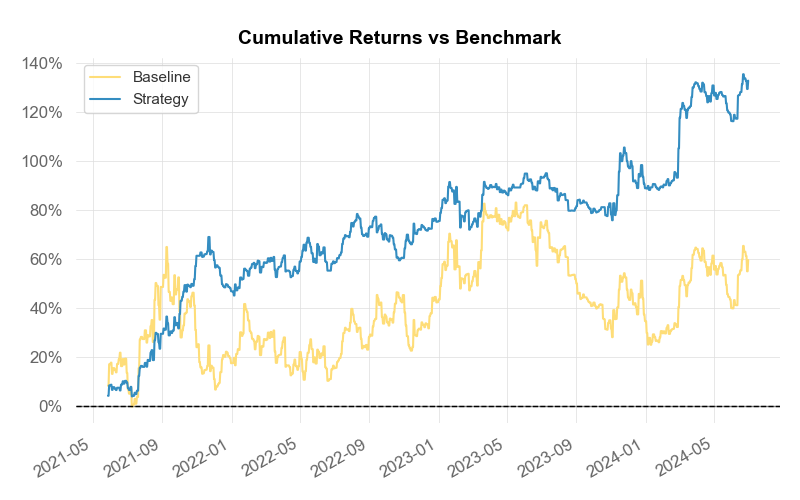
\includegraphics[width=0.9\linewidth]{headline_plots/NAV.png}% <-- put your path
\caption{Cumulative NAV: baseline vs.\ regime overlay.}
\label{fig:nav}
\end{figure}

\begin{figure}[t]
\centering
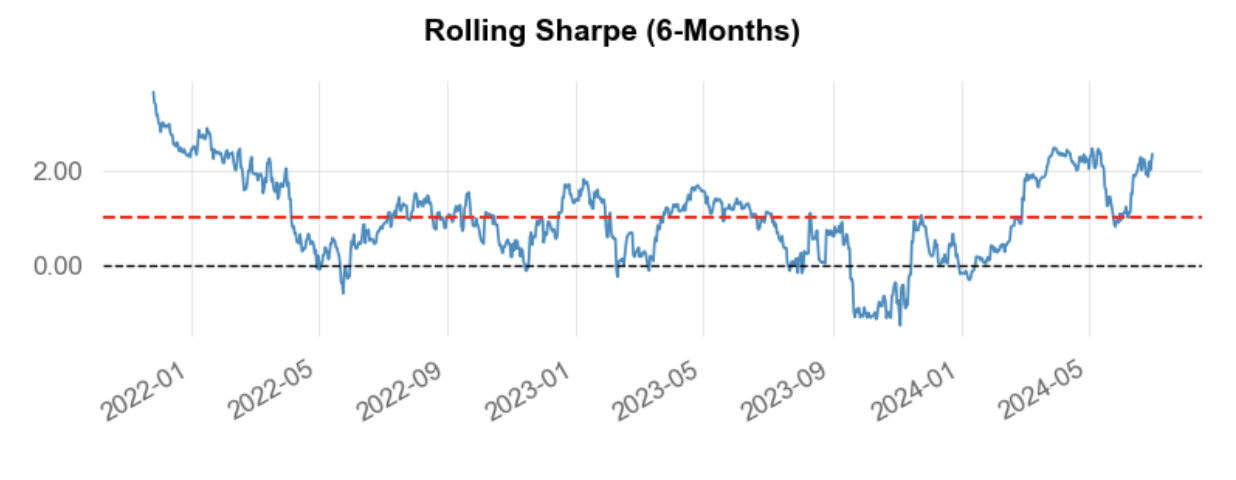
\includegraphics[width=0.9\linewidth]{headline_plots/Rolling_Sharp.png}
\caption{Rolling 6-month Sharpe for the baseline and the Overlay.}
\label{fig:roll_sharpe_6m}
\end{figure}


\begin{table}[t]
\centering
\caption{Drawdown details.}
\label{tab:diag_dd}
\small
\begin{tabular}{lcc}
\toprule
Metric & Baseline & Overlay \\
\midrule
Max DD (\%)          & -35.32 & -14.15 \\
Max DD Date          & 2021-12-03 & 2022-01-05 \\
Max DD Period Start  & 2021-09-10 & 2021-11-24 \\
Max DD Period End    & 2023-01-17 & 2022-07-19 \\
Longest DD Days      & 495 & 238 \\
\bottomrule
\end{tabular}
\end{table}

Table~\ref{tab:diag_dd} details the drawdown. The overlay cuts the peak--to--trough loss from \textbf{--35.32\%} to \textbf{--14.15\%}. It also halves time under water from \textbf{495} to \textbf{238} days. The baseline’s worst episode is long and persistent (\textbf{2021-09-10} to \textbf{2023-01-17}; trough on \textbf{2021-12-03}) and spans the 2022 downturn. The overlay’s worst spell starts later (\textbf{2021-11-24}), bottoms quickly (\textbf{2022-01-05}), and ends by mid-\textbf{2022} (\textbf{2022-07-19}). In other words, it absorbs the early-2022 selloff but exits and recovers faster. Net effect: a softer left tail and a shorter recovery horizon, consistent with the higher risk-adjusted performance.

\begin{table}[t]
\centering
\caption{EOY returns vs.\ baseline. Multiplier $=$ Strategy / Baseline; negative means opposite signs.}
\label{tab:eoy}
\small
\begin{tabular}{lrrrr}
\toprule
Year & Baseline & Strategy & Multiplier & Won \\
\midrule
2021 & 16.28\% & 46.77\% & 2.87  & $+$ \\
2022 & 21.22\% & 19.36\% & 0.91  & $-$ \\
2023 & $-5.42$\% & 7.79\% & $-1.44$ & $+$ \\
2024 & 18.54\% & 23.27\% & 1.26  & $+$ \\
\bottomrule
\end{tabular}
\end{table}

Table~\ref{tab:eoy} compares year-end returns and the multiplier (Strategy/Baseline). The overlay wins in \textbf{three of four} years---\textbf{2021}, \textbf{2023}, and \textbf{2024 (YTD)}---with multipliers of \textbf{2.87}, \textbf{-1.44}, and \textbf{1.26}. The negative multiplier in 2023 signals a sign flip (baseline \(-5.42\%\) vs.\ strategy \(+7.79\%\)). In \textbf{2022}, the multiplier is \textbf{0.91}, a mild shortfall. Overall, the overlay adds value when the baseline struggles and still provides an edge in rising markets.

\begin{table}[t]
\centering
\caption{Top-5 by Sharpe compared with baseline strategy.}
\label{tab:top5_sharpe_params}
\small
\begin{tabular}{lccccccc}
\toprule
Strategy (params) & Sharpe & CAGR & Vol (ann) & MaxDD & Calmar & Alpha (ann) & WinRate \\
\midrule
$n\_steps, n\_paths=5, 20$ & 1.460 & 0.314 & 0.201 & -0.141 & 2.161 & 0.212 & 0.215 \\
$n\_steps, n\_paths=5, 16$ & 1.006 & 0.217 & 0.218 & -0.207 & 1.046 & 0.126 & 0.216 \\
$n\_steps, n\_paths=15, 12$ & 0.892 & 0.150 & 0.173 & -0.173 & 0.863 & 0.112 & 0.155 \\
$n\_steps, n\_paths=15, 16$ & 0.853 & 0.154 & 0.188 & -0.155 & 0.994 & 0.100 & 0.157 \\
$n\_steps, n\_paths=5, 8$  & 0.816 & 0.161 & 0.210 & -0.192 & 0.841 & 0.095 & 0.214 \\
\hline
Baseline & 0.580 & 0.163 & 0.380 & -0.353 & 0.440 & 0.000 & 0.219 \\
\bottomrule
\end{tabular}
\end{table}


\section{Strategy selection and performance}\label{sec:results:top5}


% In your preamble:
% \usepackage{graphicx}

\begin{figure}[t]
  \centering
  % If you saved to images/top5_nav_union.png:
  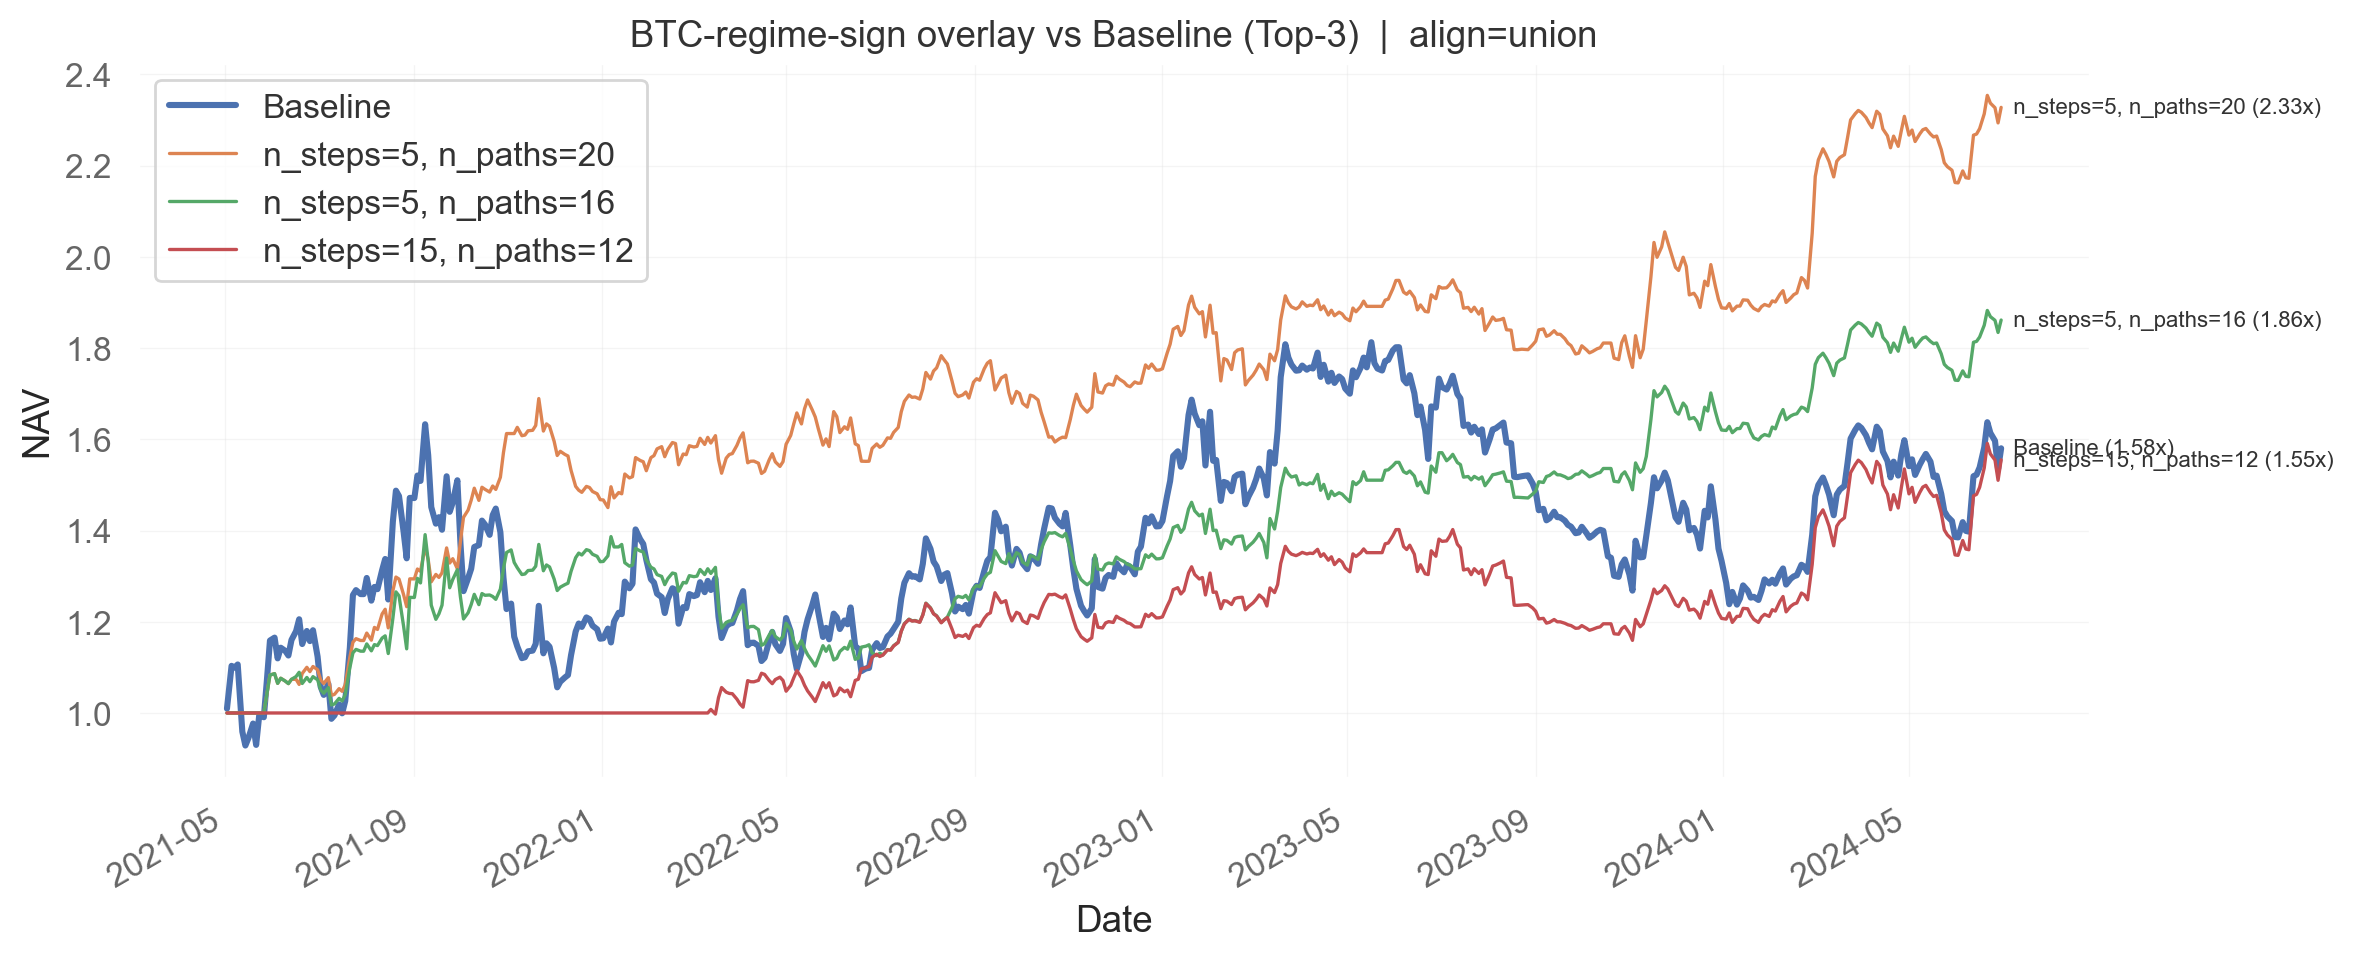
\includegraphics[width=\linewidth]{headline_plots/top3_nav_union.png}
  \caption{Top-3 NAV vs. Baseline (union-aligned). Values annotated at the last date indicate final NAV multiples.}
  \label{fig:top5_nav_union}
\end{figure}

First, we evaluate candidate parameterisations in a \emph{strict walk-forward} setup, train only on past windows and label only the current group. Then we rank each configuration by Sharpe. For context, we also report the Baseline. Throughout, we use a unified daily calendar with a crypto annualisation factor of 365. We align returns from the \emph{signal day} to the \emph{next trading day}. Rates are in decimals (e.g., 0.20 = 20\%). See Table~\ref{tab:top5_sharpe_params}.

Short windows with more paths perform best. In particular, \(n_{\text{steps}}=5\) with \(n_{\text{paths}}\in\{16,20\}\) leads. The top configuration, \(n_{\text{steps}}=5, n_{\text{paths}}=20\), reaches a Sharpe of 1.44 with annualised volatility of 0.20, maximum drawdown \(-0.14\), and Calmar 2.16. By contrast, the Baseline records a Sharpe of 0.56 and a Calmar of 0.44. Meanwhile, mid-range windows—such as \(n_{\text{steps}}=15\) with \(n_{\text{paths}}\in\{12,16\}\)—also offer a solid return-risk trade-off.

We assess significance against zero using Newey--West (HAC, Bartlett kernel; data-driven lag) t-statistics on daily excess returns (See Appendix \ref{sec:newey-west}).
We then build 95\% moving-block bootstrap confidence intervals (block = 10 days, $B=2000$) for annualized return and Sharpe on the unified calendar.
Table~\ref{tab:sig_compact} reports the Baseline and the top five overlays by Sharpe.
As shown, \emph{Overlay (5,20)} is significant versus zero; both confidence intervals lie strictly above zero.
\emph{Overlay (5,16)} is marginally significant.
By contrast, the Baseline and the remaining overlays are not significant at the 5\% level, with intervals overlapping zero.

\begin{table}[t]
\centering
\caption{Significance vs.\ zero: NW $t$ on daily mean excess, and 95\% block-bootstrap CIs. Rates in decimals (e.g., 0.20 = 20\%).}
\label{tab:sig_compact}
\small
\begin{tabular}{lccccc}
\toprule
Strategy & NW $t$ (mean) & AnnRet (pt) & AnnRet [2.5\%,97.5\%] & Sharpe (pt) & Sharpe [2.5\%,97.5\%] \\
\midrule
Baseline        & 1.29 & 0.24 & [$-0.18$, $0.90$] & 0.58 & [$-0.35$, $1.80$] \\
Overlay (5,20)  & 2.67 & 0.33 & [$0.08$,  $0.64$] & 1.46 & [$0.48$,  $2.48$] \\
Overlay (5,16)  & 2.01 & 0.24 & [$0.01$,  $0.54$] & 1.00 & [$0.13$,  $2.10$] \\
Overlay (15,12) & 1.58 & 0.15 & [$-0.05$, $0.40$] & 0.89 & [$-0.20$, $1.96$] \\
Overlay (15,16) & 1.54 & 0.16 & [$-0.05$, $0.43$] & 0.85 & [$-0.18$, $1.88$] \\
Overlay (5,8)   & 1.53 & 0.17 & [$-0.07$, $0.47$] & 0.81 & [$-0.25$, $1.90$] \\
\bottomrule
\end{tabular}
\end{table}

Several other settings (e.g., \(n_{\text{steps}}\in\{8,10\}\)) are mediocre or negative in this sample and are omitted. In practice, implementation should also account for switching frequency and transaction costs (see the switch-rate diagnostics), since these frictions affect net returns and capacity. Overall, the walk-forward state signal, when combined with our overlay, improves risk-adjusted performance, with “shorter steps + more paths” as the most effective pattern in this dataset.


\section{Transaction-cost modeling and impact}\label{sec:tc}

We model transaction costs in a simple, transparent way that matches our portfolio construction and evaluation. First, on each trading day \(t\) we form target portfolio weights \(w_t\) (long equal-weight followers; short equal-weight leaders). Next, we proxy trading volume with the absolute change in target weights.
\[
\text{turnover}_t = \sum_i \lvert w_{t,i} - w_{t-1,i}\rvert.
\]
We then apply a per-side fee of \(c\) basis points to this turnover, which yields the daily cost
\[
\text{cost}_t = (c\times 10^{-4})\;\text{turnover}_t.
\]
Consequently, we compute net returns in \emph{simple-return} space as
\(r^{\text{net}}_t = r^{\text{gross}}_t - \text{cost}_t\).
We charge for the first trade (initial portfolio formation) and use the \emph{target-diff} mechanic. %For completeness, a \emph{full-rebalance} variant that also offsets drift back to equal weights produces higher costs and is reported when noted.

\begin{table}
\caption{Baseline transaction-cost sensitivity (per side, applied to target-weight changes).}
\label{tab:baseline_tc}
\small
\centering
\begin{tabular}{rrrrr}
\toprule
Cost (bps/side) & Sharpe & AnnRet (\%) & Vol (\%) & MaxDD (\%) \\
\midrule
5   & 0.323  & 5.07   & 40.98 & -42.36 \\
10  & -0.015 & -8.56  & 40.99 & -58.57 \\
25  & -1.026 & -39.77 & 41.15 & -86.30 \\
\bottomrule
\end{tabular}
\end{table}

\begin{table}
\caption{Transaction-cost sensitivity. Costs are per side, applied to target-weight changes.}
\label{tab:tc_sensitivity_reduced}
\small
\centering
\begin{tabular}{lrrrr}
\toprule
Strategy (params) & Sharpe & AnnRet (\%) & Vol (\%) & MaxDD (\%) \\
\midrule
\multicolumn{5}{l}{\emph{Cost = 5 bps/side}}\\
\params{5}{20} & 1.052 & 26.82 & 25.70 & -22.98 \\
\params{5}{16} & 0.628 & 14.24 & 26.86 & -34.98 \\
\params{15}{12} & 0.475 & 9.45 & 26.12 & -31.18 \\
\params{15}{16} & 0.561 & 11.88 & 25.96 & -27.17 \\
\params{5}{8} & 0.485 & 9.81 & 26.50 & -26.90 \\
\addlinespace
\multicolumn{5}{l}{\emph{Cost = 10 bps/side}}\\
\params{5}{20} & 0.672 & 15.03 & 25.68 & -32.08 \\
\params{5}{16} & 0.289 & 4.28 & 26.82 & -39.22 \\
\params{15}{12} & 0.122 & -0.19 & 26.13 & -36.51 \\
\params{15}{16} & 0.197 & 1.78 & 25.96 & -33.31 \\
\params{5}{8} & 0.103 & -0.76 & 26.50 & -34.76 \\
\addlinespace
\multicolumn{5}{l}{\emph{Cost = 25 bps/side}}\\
\params{5}{20} & -0.466 & -14.21 & 25.79 & -65.20 \\
\params{5}{16} & -0.732 & -20.73 & 26.84 & -63.57 \\
\params{15}{12} & -0.931 & -24.35 & 26.28 & -68.04 \\
\params{15}{16} & -0.892 & -23.39 & 26.07 & -66.77 \\
\params{5}{8} & -1.038 & -26.80 & 26.62 & -68.02 \\
\bottomrule
\end{tabular}
\end{table}

Costs erode performance roughly in line with annualised turnover. For the Baseline (Table~\ref{tab:baseline_tc}), sharpe drops from \(0.58\) at \(0\) bps to \(0.32\) at \(5\) bps, and turns negative by \(10\) bps. Therefore, the break-even lies between \(5\) and \(10\) bps under the \emph{target-diff} mechanic. By contrast, the best overlay configurations (Table~\ref{tab:tc_sensitivity_reduced}) suffer a milder hit thanks to lower average daily turnover (\(\sim1.16\)–\(1.30\) vs.\ Baseline \(1.77\)). For example, \(n_{\text{steps}}=5, n_{\text{paths}}=20\) remains attractive at \(5\)–\(10\) bps (Sharpe \(1.05 \to 0.67\)), yet performance compresses sharply beyond \(25\) bps. As expected, volatility is largely unchanged across bps grids, while maximum drawdowns deepen as net returns are shaved each day. At high frictions, all configurations become economically unviable, and NAVs converge toward unity.


% --------- OPTIONAL (comment out if not needed now) ----------
% \subsection{Ablations (compact)}
% \begin{table}[t]
% \centering
% \caption{Key ablations. Effect on Sharpe / MDD / turnover.}
% \begin{tabular}{lrrr}
% \toprule
% Variant & $\Delta$Sharpe & $\Delta$Max DD (pp) & $\Delta$Turnover (pp/day) \\
% \midrule
% No preserve-hedge &  &  &  \\
% No apply-to-leaders &  &  &  \\
% abs\_rel\_quantile=0.8 &  &  &  \\
% \bottomrule
% \end{tabular}
% \end{table}

%% ----------------------------------------------------------------
%% Chapter — Discussion (revised: ≤3 sections, no summary)
%% ----------------------------------------------------------------
\chapter{Discussion}\label{Chapter:Discussion}

This chapter interprets the evidence rather than re-reporting it. We explain what the regime-aware overlay changes relative to the lead--lag hedge, why those changes plausibly work, and how robust and implementable they look. We then state the main limitations and sketch next steps. Conventions and headline metrics appear in Section \ref{sec:results:headline}; we refer to them without repeating details.

\section{Interpreting the findings}\label{sec:disc:interpret}

The overlay improves return per unit risk while \emph{holding participation constant} (Table~\ref{tab:main}). Therefore, the gain comes from selection and timing, not leverage. Figure~\ref{fig:nav} shows a smoother equity curve; Table~\ref{tab:diag_dd} shows a softer left tail and faster recovery. Figure~\ref{fig:roll_sharpe_6m} adds the dynamic view: the overlay spends more time above a 6-month Sharpe of 1 and shortens the negative pockets around 2022. In calendar time (Table~\ref{tab:eoy}), the overlay helps most when the baseline is misaligned or when regime shifts are sharp; when the baseline is already onside, marginal gains shrink.

Why does this happen? The baseline is a fixed long-followers/short-leaders hedge. The overlay routes that hedge through state labels linked to BTC path geometry. In favourable states it tilts toward assets that propagate the anchor; in adverse states it flips the sign while \emph{preserving} the hedge. Gross exposure stays similar, but composition rotates with the state. This reduces whipsaws and trims losses early when conditions turn.

\section{Sensitivity and implementability}\label{sec:disc:robust}

Across strict walk-forward runs, short windows with more paths dominate (Table~\ref{tab:top5_sharpe_params}). In particular, \(n_{\text{steps}}{=}5\) with \(n_{\text{paths}}\in\{16,20\}\) balances sensitivity and stability; mid-length settings improve on the baseline but with lower Sharpe. This pattern is consistent with a bias–variance trade-off: long windows blur turning points, while too few paths raise variance in the distance estimates.

Statistical checks support a cautious reading. Against zero, the top configuration is significant and its block-bootstrap confidence intervals exclude zero; the next is marginal. However, after White’s Reality Check (WRC) and Hansen’s SPA (SPA), we cannot reject no outperformance relative to the baseline (overall \(p\approx0.66\); see Table~\ref{tab:wrc_spa}). Hence we emphasise absolute improvement and drawdown control, not a guaranteed beat of the baseline.

Finally, implementability hinges on turnover. Costs erode performance roughly in proportion to annualised turnover. The baseline breaks even between 5–10 bps/side (Table~\ref{tab:baseline_tc}). The best overlay remains attractive at 5–10 bps because average turnover is lower, but performance compresses beyond 25 bps (Table~\ref{tab:tc_sensitivity_reduced}). Simple throttles help in practice: skip small basket changes, increase rebalance spacing in high-noise states, and cap participation relative to liquidity.

\section{Limitations and next steps}\label{sec:disc:limits}

Scope comes first. The sample is daily and limited to \sampleStart{}–\sampleEnd{} with a crypto-centric anchor; external validity to other regimes or asset classes is not guaranteed. Second, the single-anchor design risks omitted-state bias if leadership rotates outside BTC; multi-anchor or hierarchical states are a natural extension. Third, several hyperparameters are fixed (kernel scale, order, regularisation). Mis-scaling can over- or under-smooth geometry, and unbiased MMD raises variance in small training windows.

Label construction also matters. Voting over the last \(k\) groups reduces jitter but adds lag; close calls near turning points can flip. Lead--lag compression to a row-mean discards pairwise uncertainty and can over-reward near-ties in lag choice. Data handling imposes further constraints: winsorisation trims extremes; funding/borrow and market impact are simplified; reported headline metrics are gross of costs unless stated.

Finally, inference carries model-selection risk. Hyperparameters were chosen plausibly rather than via nested, walk-forward cross-validation. Multiple testing remains a threat despite our compact grid; WRC/SPA results underscore that caution. Next steps follow directly: extend to \emph{multi-anchor} regimes; add \emph{uncertainty-aware} scaling that gates gross exposure by state confidence; incorporate execution-aware controls (impact, latency, borrow/funding); and formalise selection with step-down SPA or a model-confidence set.

%% ----------------------------------------------------------------
%% Chapter — Conclusion (no sections)
%% ----------------------------------------------------------------
\chapter{Conclusion}\label{Chapter:Conclusion}

This dissertation studied how \emph{path-wise} information extracted by signature methods can detect market regimes in a strict walk–forward setting and improve a signature-based lead--lag hedge. We started from daily BTC data from \sampleStart{} to\sampleEnd{} and built backward-looking regime labels with a signature–kernel MMD on rolling path groups and combined them with a rolling signature lead--lag matrix across assets. We then overlaid the baseline hedge (long followers / short leaders) with state-conditioned basket selection keyed to the BTC anchor, while preserving the hedge structure.

The overlay raises return per unit risk at the same market participation. Cumulative return increases from 59.53\% to 132.78\%. Sharpe rises from 0.58 to 1.46 and Sortino from 0.90 to 2.46, while annualised volatility falls from 38.09\% to 20.06\% (Table~\ref{tab:main}). Drawdowns are shallower and shorter: the maximum improves from --35.32\% to --14.15\%, and underwater time halves from 495 to 238 days (Table~\ref{tab:diag_dd}). Year-by-year results show three wins out of four (2021, 2023, 2024 YTD) and a mild shortfall in 2022 (Table~\ref{tab:eoy}). Across strict walk–forward runs, shorter windows with more paths perform best; \(n_{\text{steps}}{=}5\) with \(n_{\text{paths}}\in\{16,20\}\) dominates neighbouring settings (Table~\ref{tab:top5_sharpe_params}). Statistical checks are consistent with a cautious reading: the top configuration is significant versus zero and its block-bootstrap CIs exclude zero (Table~\ref{tab:sig_compact}), whereas we do not reject no outperformance relative to the baseline (Table~\ref{tab:wrc_spa}). Costs matter but do not erase the edge at realistic frictions: the baseline breaks even around 5–10 bps/side; the top overlay remains attractive at 5–10 bps and degrades beyond 25 bps (Tables~\ref{tab:baseline_tc}–\ref{tab:tc_sensitivity_reduced}).

The mechanism is relatively simple. The overlay does not lever up, extend holding time, or chase beta. It \emph{routes} the same hedge through regime information. In bull states it favours names that co-move with the anchor; in bear states it flips signs; in neutral states it scales. Gross exposure stays similar, but composition rotates with the state. This reduces whipsaws, trims left-tail losses, and speeds recovery.

Methodologically and empirically, the work contributes four elements: (i) a strict walk–forward regime detector based on signature–kernel MMD with medoid mapping to bull/neutral/bear labels; (ii) a signature-based lead--lag matrix that captures directional, order-sensitive dependence and a transparent baseline hedge; (iii) a \emph{regime-aware overlay} that preserves the hedge while gating baskets by an anchor-signed relation; and (iv) a reproducible evaluation protocol with unified calendar alignment, signal-to-execution timing, turnover-based costs, and diagnostics for drawdowns, yearly performance, and parameter sensitivity.

The conclusions are bounded. The sample is daily and crypto-centric over \sampleStart{}–\sampleEnd{}; external validity to other periods or asset classes is not guaranteed. A single BTC anchor can miss leadership outside crypto. Several hyperparameters are fixed (kernel scale, order, regularisation), and unbiased MMD raises variance in small training windows. Rolling votes reduce label jitter but add lag near turning points. Row-mean leadership compresses pairwise uncertainty, and lag maximisation can overfit short windows. Frictions—fees, funding/borrow, impact—are modelled parsimoniously; net results depend on venue microstructure. Finally, model selection risk remains despite a compact grid; the WRC/SPA outcome underlines that caution.

Promising extensions follow naturally. Multi-anchor or hierarchical regimes could generalise the design beyond BTC. Probabilistic states would allow confidence-weighted scaling of exposure and trades. Cost-aware construction, such as turnover penalties, participation caps, and state-dependent rebalance spacing, could harden net performance. Kernel approximations and streaming clustering would improve scalability. Broader data horizons would test temporal and frequency robustness.

In summary, path-wise regime information can be combined with directional lead--lag structure to produce a \emph{regime-aware hedge} that is more resilient and capital efficient than its unconditional counterpart. The approach is modular: path features, regime mapping, and portfolio rules can be swapped independently. This makes the framework a practical template for bringing modern geometric time-series tools into risk-managed trading.

\appendix
%% ----------------------------------------------------------------
%% AppendixA.tex
%% ---------------------------------------------------------------- 
\begin{longtable}{@{}rll@{}}
\caption{Asset list with full names and tickers}\label{tab:assets}\\
\toprule
No. & Full name & Ticker \\
\midrule
\endfirsthead
\toprule
No. & Full name & Ticker \\
\midrule
\endhead
\bottomrule
\endfoot

1  & Oasis Network        & \texttt{ROSE} \\
2  & Ankr                 & \texttt{ANKR} \\
3  & VeChain              & \texttt{VET} \\
4  & NEAR Protocol        & \texttt{NEAR} \\
5  & Ethereum             & \texttt{ETH} \\
6  & EOS                  & \texttt{EOS} \\
7  & BakeryToken          & \texttt{BAKE} \\
8  & The Graph            & \texttt{GRT} \\
9  & Reef                 & \texttt{REEF} \\
10 & Injective            & \texttt{INJ} \\
11 & Filecoin             & \texttt{FIL} \\
12 & Polygon              & \texttt{MATIC} \\
13 & Bitcoin Cash         & \texttt{BCH} \\
14 & IOST                 & \texttt{IOST} \\
15 & Chromia              & \texttt{CHR} \\
16 & MultiversX           & \texttt{EGLD} \\
17 & Hedera               & \texttt{HBAR} \\
18 & Zilliqa              & \texttt{ZIL} \\
19 & Algorand             & \texttt{ALGO} \\
20 & Dent                 & \texttt{DENT} \\
21 & Dash                 & \texttt{DASH} \\
22 & My Neighbor Alice    & \texttt{ALICE} \\
23 & IOTA                 & \texttt{IOTA} \\
24 & Chainlink            & \texttt{LINK} \\
25 & Tezos                & \texttt{XTZ} \\
26 & Loopring             & \texttt{LRC} \\
27 & Harmony              & \texttt{ONE} \\
28 & Solar                & \texttt{SXP} \\
29 & Kava                 & \texttt{KAVA} \\
30 & Axie Infinity        & \texttt{AXS} \\
31 & Cardano              & \texttt{ADA} \\
32 & Solana               & \texttt{SOL} \\
33 & Ontology             & \texttt{ONT} \\
34 & Ethereum Classic     & \texttt{ETC} \\
35 & Decentraland         & \texttt{MANA} \\
36 & Synthetix            & \texttt{SNX} \\
37 & Zcash                & \texttt{ZEC} \\
38 & Conflux              & \texttt{CFX} \\
39 & Yearn Finance        & \texttt{YFI} \\
40 & Waves                & \texttt{WAVES} \\
41 & Litecoin             & \texttt{LTC} \\
42 & Chiliz               & \texttt{CHZ} \\
43 & Stellar              & \texttt{XLM} \\
44 & COTI                 & \texttt{COTI} \\
45 & Polkadot             & \texttt{DOT} \\
46 & OMG Network          & \texttt{OMG} \\
47 & SushiSwap            & \texttt{SUSHI} \\
48 & Fantom               & \texttt{FTM} \\
49 & BNB                  & \texttt{BNB} \\
50 & Uniswap              & \texttt{UNI} \\
51 & Stacks               & \texttt{STX} \\
52 & THORChain            & \texttt{RUNE} \\
53 & Theta Network        & \texttt{THETA} \\
54 & Holo                 & \texttt{HOT} \\
55 & 1inch                & \texttt{1INCH} \\
56 & Fetch.ai             & \texttt{FET} \\
57 & Kusama               & \texttt{KSM} \\
58 & Smooth Love Potion   & \texttt{SLP} \\
59 & Curve DAO Token      & \texttt{CRV} \\
60 & IoTeX                & \texttt{IOTX} \\
61 & Bitcoin              & \texttt{BTC} \\
62 & Avalanche            & \texttt{AVAX} \\
63 & Enjin Coin           & \texttt{ENJ} \\
64 & PancakeSwap          & \texttt{CAKE} \\
65 & XRP                  & \texttt{XRP} \\
66 & TRON                 & \texttt{TRX} \\
67 & Cosmos               & \texttt{ATOM} \\
68 & Aave                 & \texttt{AAVE} \\
69 & Dogecoin             & \texttt{DOGE} \\
70 & Neo                  & \texttt{NEO} \\
71 & The Sandbox          & \texttt{SAND} \\
72 & Qtum                 & \texttt{QTUM} \\
\end{longtable}

% Notation
% D in R^{G x G}, symmetric; t_i end times; raw boundary t_train^raw; horizon H
% Safe boundary: t_train^safe = t_train^raw - H
\iffalse
\textbf{Training set:}\quad
I_{\text{train}} = \{\, i : t_i \le t_{\text{train}}^{\text{safe}} \,\}.

\textbf{Clustering \& medoids:}\quad
\text{Cluster } D[I_{\text{train}}, I_{\text{train}}] \to \{C_k\}_{k=1}^K,\quad
m_k = \arg\min_{j \in C_k} \sum_{i \in C_k} D_{ij}.

\textbf{Forward return (H steps) for } i \in C_k:\quad
r_H(i) = \frac{P(t_i + H) - P(t_i)}{P(t_i)}.

\textbf{Discrete direction:}\quad
\mathrm{dir}(i) =
\begin{cases}
\text{Bull}, & r_H(i) \ge \tau_{\text{pos}},\\
\text{Bear}, & r_H(i) \le -\tau_{\text{neg}},\\
\text{Sideways}, & \text{otherwise.}
\end{cases}

\textbf{Cluster semantic (majority vote):}\quad
L_k \in \{\text{Bear, Sideways, Bull}\}
\text{ from } \{\mathrm{dir}(i): i \in C_k\}.
\text{ (Tie-break by sign of } \overline{r_H} \text{ or medoid’s label.)}

\textbf{Prototype dictionary:}\quad
\mathcal{M} = \{(m_k, L_k)\}_{k=1}^K.

\textbf{Assignment on all groups:}\quad
c(g) = \arg\min_k D_{g, m_k}, \qquad
\widehat{\mathrm{dir}}(g) = L_{c(g)}.

\textbf{Rolling vote (optional):}\quad
\widetilde{\mathrm{dir}}(g) = \operatorname{mode}\big(\widehat{\mathrm{dir}}(g-k_{\text{vote}}+1),\dots,\widehat{\mathrm{dir}}(g)\big).

\textbf{Daily mapping:}\quad
\text{Expand group labels over their date spans to obtain a daily series.}

\textbf{No-leakage:}\quad
\text{Only use } i \text{ with } t_i + H \le t_{\text{train}}^{\text{raw}}.
\text{ Equivalently, } t_{\text{train}}^{\text{safe}} = t_{\text{train}}^{\text{raw}} - H.
\fi

\section{Signature Theory}

The signature of a path is a mathematical object that originates from rough path theory (Lyons, 1998). 
Given a $d$-dimensional continuous path $X : [0,T] \to \mathbb{R}^d$, the signature is defined as the infinite collection of \emph{iterated integrals} of the path: 
\[
S(X) = \left( 1, S^{(1)}(X), S^{(2)}(X), S^{(3)}(X), \dots \right),
\]
where the $k$-th level signature term is
\[
S^{(k)}(X) = \int_{0 < t_1 < \cdots < t_k < T} dX_{t_1} \otimes dX_{t_2} \otimes \cdots \otimes dX_{t_k}.
\]

At the first level ($k=1$), the signature reduces to the net increment of the path:
\[
S^{(1)}(X) = X_T - X_0.
\]
At the second level, we obtain quadratic information that encodes the order of movements:
\[
S^{(2)}(X) = \int_{0 < t_1 < t_2 < T} dX_{t_1} \otimes dX_{t_2},
\]
which captures how one coordinate of the path leads or lags another. Higher-order terms generalise this to more complex dependencies.

Two properties make the signature especially powerful. First, \textbf{Chen’s identity} guarantees that the signature of a concatenated path can be decomposed into signatures of its segments, making it suitable for sequential data. Second, under mild conditions, the \textbf{signature uniquely characterises the path} up to so-called ``tree-like'' equivalence, meaning that it retains essentially all the information of the original trajectory (Lyons, 1998; Hambly and Lyons, 2010). 

Since the full signature is infinite-dimensional, in practice one truncates it at depth $m$. 
The dimension of the truncated signature grows polynomially:
\[
\dim S^{\leq m}(X) = \sum_{k=0}^m d^k,
\]
which means that for even moderate $d$ and $m$, the feature space becomes high-dimensional. This motivates careful choices of truncation level and path embedding.


Financial time series such as asset prices are inherently sequential and path-dependent. Traditional summary statistics---such as mean, variance, or simple autocorrelations---capture only coarse properties of the distribution. In contrast, signature features encode the order and interaction of movements at multiple scales, making them particularly suitable for detecting subtle temporal structures.  
For example, second-order signature terms can reflect lead--lag effects between variables, while higher-order terms can characterise nonlinear dependencies that may indicate regime shifts.  
This ability to represent paths beyond linear summary statistics makes the signature method a natural candidate for regime detection in financial markets.

\subsection{Maximum Mean Discrepancy (MMD)}

Once features are extracted, the problem of regime detection becomes a problem of identifying distributional changes over time. To this end, we adopt the \textbf{Maximum Mean Discrepancy (MMD)} as a non-parametric two-sample test (Gretton et al., 2012).  

Given two sets of observations $X = \{x_i\}_{i=1}^n$ and $Y = \{y_j\}_{j=1}^m$ in feature space $\mathcal{X}$, the squared MMD between their distributions $P$ and $Q$ is defined as:
\[
\mathrm{MMD}^2(P,Q;\mathcal{H}) = \sup_{f \in \mathcal{H}, \|f\|_{\mathcal{H}} \leq 1} \left( \mathbb{E}_{x \sim P}[f(x)] - \mathbb{E}_{y \sim Q}[f(y)] \right)^2,
\]
where $\mathcal{H}$ is a reproducing kernel Hilbert space (RKHS).  

In practice, with a kernel function $k(\cdot, \cdot)$, the unbiased empirical estimate is:
\[
\widehat{\mathrm{MMD}}^2(X,Y) = \frac{1}{n(n-1)} \sum_{i \neq i'} k(x_i, x_{i'}) + \frac{1}{m(m-1)} \sum_{j \neq j'} k(y_j, y_{j'}) - \frac{2}{nm} \sum_{i,j} k(x_i, y_j).
\]

If $\widehat{\mathrm{MMD}}^2$ is large, it indicates that the two sets of observations likely come from different distributions, i.e., a regime shift. The choice of kernel (e.g., Gaussian RBF) controls the sensitivity to local vs. global changes.



\subsection{Construction of Distance Matrices}

To perform clustering, we require a distance measure between different segments of the BTC price path. 
The first step is \textbf{subpath extraction}. The original time series is divided into overlapping subpaths of fixed length $n_{\text{steps}}$. Each subpath represents the local dynamics of the market over a short horizon, ensuring that temporal dependencies are preserved.

Next, we introduce a \textbf{grouping stage}. Instead of treating each subpath individually, we aggregate $n_{\text{paths}}$ consecutive subpaths into groups. This reduces the effect of noise and yields more stable representations of local behaviour. Each group can be regarded as a local distribution of path features.

Finally, we compute \textbf{pairwise distances} between groups. After transforming each path using the signature representation, we employ a Maximum Mean Discrepancy (MMD)–based metric to quantify the distributional difference between two groups. The outcome is a symmetric distance matrix $D \in \mathbb{R}^{G \times G}$, where $G$ denotes the number of groups. This distance matrix serves as the input for subsequent clustering, enabling the identification of distinct market regimes.
\backmatter
\bibliographystyle{ecs}
\bibliography{ECS}
\end{document}
%% ----------------------------------------------------------------
